\documentclass[11pt,ngerman]{scrartcl}

% standard packages
\usepackage[utf8]{inputenc}  % input in UTF-8
\usepackage[T1]{fontenc}  % output in T1 fonts (westeuropäische Codierung)
\usepackage{lmodern}  % latin modern fonts
\usepackage[ngerman]{babel}  % deutsches Sprachpaket, neue Rechtschreibung

% Seitensetup
\usepackage{scrlayer-scrpage}  % Seitenformatierung durch KOMA-interne Optionen
\usepackage[top=4cm, bottom=4cm]{geometry}  % Seitengeometrie (kann durch KOMA ersetzt werden, hab ich aber nicht geschafft)
\usepackage[hypcap=false]{caption, subcaption}  % caption editing - hypcap warning with hyperref
\usepackage{array}  % table editing

% additional packages
\usepackage{amsmath, amssymb, amstext}  % math packages (American Math Society)
\usepackage{bm}
\usepackage{icomma}  % Kommata in Dezimalzahlen verursachen keinen Abstand mehr
\usepackage{graphicx}  % Bilder einfügen
\usepackage{float} %Bilder placement
\usepackage{pdfpages}  % PDF als vollständige Seiten einfügen
\usepackage{lastpage}  % referenziert die letzte Seite
\usepackage[separate-uncertainty=true]{siunitx}  % bessere Darstellung von Einheiten
\usepackage{makecell} %Dicke Tabellenstriche
\usepackage{longtable}
\usepackage{booktabs}
%\usepackage{datatool}
\usepackage[hidelinks]{hyperref}  % hyperref verlinkt Referenzen - hidelinks entfernt borders um links

% package setups
% Kopf- und Fußzeile durch KOMA
\pagestyle{scrheadings}  % KOMA darf entscheiden
\clearpairofpagestyles  % reset
\setkomafont{pageheadfoot}{\normalfont}  % Standardschrift in Kopf- und Fußzeile
\captionsetup{format=plain, font=small, labelfont=bf} %Better caption, Abbildung ist FETT
%\setlength{\headheight}{27.2pt}  % benötigte Höhe Kopfzeile (warning von scrlayer-scrpage, wird aber automatisch so gerendert, falls diese Option weggelassen wird)
\ihead{Brennweite \\ dünner Linsen}  % Kopf links %Todo Titel ändern
\chead{\textsc{Philipp} Maximilian \\ \textsc{Stark} Matthias}  % Kopf Mitte %Todo Name ändern
\ohead{12 November 2021}  % Kopf rechts %Todo Datum ändern
\cfoot{\pagemark \, / \pageref{LastPage}}  % Fuß Mitte

% Table of Contents
\DeclareTOCStyleEntry{dottedtocline}{section}  % KOMA intern - Inhaltsverzeichnis mit Punkten (nur sections)

%Overbar setup
\newcommand{\overbar}[1]{\mkern 1.5mu\overline{\mkern-1.5mu#1\mkern-1.5mu}\mkern 1.5mu}
% SI
\sisetup{locale = DE}  % deutschsprachige SI-Konvention
\sisetup{quotient-mode = fraction}
\sisetup{per-mode = fraction}
\DeclareSIUnit\px{px}
\DeclareSIUnit\strich{|||}

% citation
\usepackage{csquotes}
%\usepackage[backend=biber]{biblatex}
\usepackage[backend=biber]{biblatex}
\addbibresource{linsen.bib} %Todo .bib befüllen zb.: mit JabRef (Empfehlung der Redaktion)

%Eigene Commands
\newcommand{\der}[2]{\frac{\mathrm{d}#1}{\mathrm{d}#2}}
\newcommand{\pder}[2]{\frac{\partial #1}{\partial #2}}

%\noindent für ges
\setlength{\parindent}{0pt}


\begin{document}

\includepdf{Deckblatt_labor2.pdf}
\tableofcontents
\newpage

\section{Aufgabenstellung\label{Auf0}}

\begin{itemize}
	\item Justieren der optischen Anordnung mittels Laser und Lochblende.

	\item Die Brennweite einer dünnen Sammellinse ist nach (3.1) zu messen (10 verschiedene Messungen!).
	      Linsen werden vom Betreuer ausgegeben. Es ist die volle Länge der optischen Bank auszunutzen,
	      dann den Schirm um jeweils 10 cm in Richtung Objekt verschieben und Bild erneut
	      scharfstellen. Für 10 verschiedene Abstände $f < g < 2f$ ist der zugehörige Bildabstand
	      $b$ im Diagramm $1/b$ als Funktion von $1/g$ aufzutragen. Gleicher, geeigneter Maßstab für
	      x- und y-Achse! Die Ausgleichskurve wird eine zur ersten Mediane senkrechte Gerade, die
	      auf der Ordinaten- und auf der Abszissenachse jeweils gleiche Strecken von der Länge der
	      reziproken Brennweite $1/f$ abschneidet. Die Maßzahl der Brechkraft $D = 1/f$ (in Dioptrien)
	      kann unmittelbar an der Achse abgelesen werden. Die derart erhaltene Brennweite ist
	      mit der aus den Einzelmessungen bestimmten Brennweite zu vergleichen.

	\item Für 5 verschiedene Gesamtabstände a ist die Brennweite derselben Linse nach dem Bessel'schen
	      Verfahren (3.2) zu kontrollieren.

	\item Es ist nach (3.3.1) die Brennweite einer Zerstreuungslinse zu messen (10 verschiedene
	      Messungen!).
	      Es sind 10 Messungen für verschiedene $g_0$, $b$ durchzuführen. Kontrolle der Brennweite nach
	      (3.3.2).

	\item Versuchen Sie, ob Sie einige Linsenfehler durch geeignetes Experimentieren darstellen
	      können.

\end{itemize}

\newpage

\section{Grundlagen}
Grundlagen wurden von den Vorlagen entnommen \cite{linsenvorlage}.

Eine ``ideale`` optische Abbildung besteht darauf, dass ein Teil, der von einem Gegenstandspunkt
$P$ (Objektpunkt) ausgehenden Lichtwellenzüge (oft als Lichtwellen bezeichnet) durch ein optisches
System (Linsen, Spiegel, Objektive) erfasst und in einem Bildpunkt $P'$ wieder vereinigt
wird (siehe \autoref{fig:abb1}). Das Bild ist dann mit dem Gegenstand konform (winkeltreu). Sind die
Abmessungen von Gegenstands- bzw. Bildgröße, Linsen- bzw. Spiegelgröße groß gegenüber der
Lichtwellenlänge, so ergibt sich eine Vereinfachung der optischen Abbildung insofern, als die
Wellennatur des Lichtes nicht berücksichtigt werden muss. Man gelangt zur sogenannten geometrischen
Optik, der das Prinzip von Fermat vorangestellt werden soll:

\vspace{2mm}

Jeder Lichtstrahl ausgehend von einem Objektpunkt wählt seinen Weg zu einem
anderen Punkt (Bildpunkt) derart, dass die dafür erforderliche Zeit ein Minimum
wird.

\vspace{2mm}

Mit diesem Prinzip lassen sich die Gesetze der Brechung, der Reflexion und der optischen Abbildung
herleiten. Weiters bekommt der Brechungsindex $n$ als ``Verzögerungsfaktor der Lichtgeschwindigkeit
in dem betreffenden Medium`` eine anschauliche Bedeutung (siehe Demtröder
Band 2 Kapitel 8.1).
Unter bestimmten Voraussetzungen kann eine Sammellinse einen Gegenstandspunkt in einen
Bildpunkt abbilden. Dazu werden die Gegenstandsweite $g$, die Bildweite $b$ und die Brennweite
$f$ benötigt. Der Zusammenhang zwischen $g$, $b$ und $f$ ist durch die Laplace'sche- und die
Newton'sche Abbildungsgleichung gegeben (siehe Demtröder Band 2, Kap. 9).

\begin{center}
	\begin{minipage}[t]{\textwidth}
		\centering
		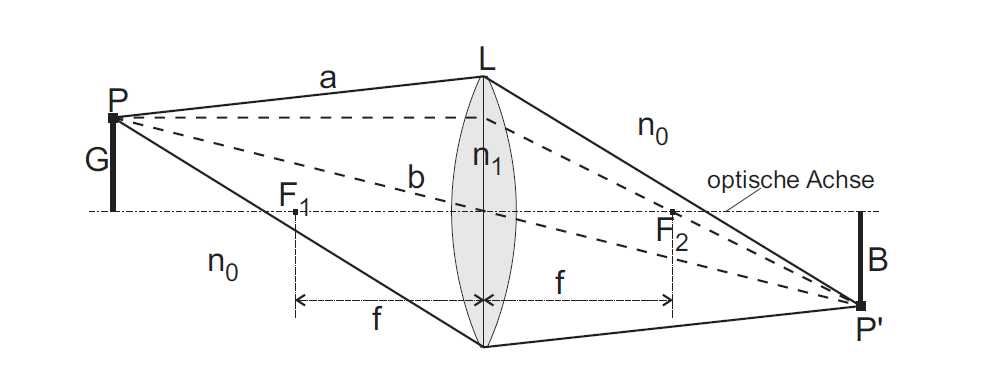
\includegraphics[width=\textwidth]{abb1}
		\captionbelowof{figure}{Gesamtbündeldarstellung der reellen Abbildung eines Objektpunktes auf den Bildpunkt
			bei einer Sammellinse. $G$ Gegenstand, $B$ Bild, $L$ Linse, $P$ Objektpunkt, $f$ Brennweite,
			$P'$ Bildpunkt, $F_1$, $F_2$ Brennpunkte, $n_0$ = 1 Brechungsindex Vakuum, $n_1$ Brechungsindex Linsenmedium,
			$a$, $b$ Lichtwege, $c_0 \approx 3 \times 10^{8}$ m/s Vakuumlichtgeschwindigkeit, $n$ Brechungsindex,
			Brechungskoeffzient oder Brechzahl, $c = c_0 /n$ Lichtgeschwindigkeit im Medium mit der Brechzahl
			$n$, $n_1 = c_0 / c_1$ Brechzahl Medium 1 mit Lichtgeschwindigkeit $c_1$.}
		\label{fig:abb1}
	\end{minipage}
\end{center}



\newpage

\section{Versuchsanordnung}\label{sec:Versuchsanordnung}

\subsection{Laplace'sche Methode}

Durch Messen von $g$ und $b$ bei
``scharfer`` Abbildung kann die Brennweite ``f`` dünner Sammellinsen
aus der Laplace'schen Abbildungsgleichung bestimmt werden:

\begin{equation}
	\frac{1}{f} = \frac{1}{g} + \frac{1}{b}
\end{equation}

Die Scharfstellung erfolgt bei Beleuchtung des Objektes mit weißem Licht und der Verwendung
von unkorrigierten Linsen. Beim Ablesen der Weite auf der Messlatte ist auf mögliche Diskrepanzen
der Reitermarken mit den entsprechenden Ebenen zu achten.

\begin{center}
	\begin{minipage}[t]{\textwidth}
		\centering
		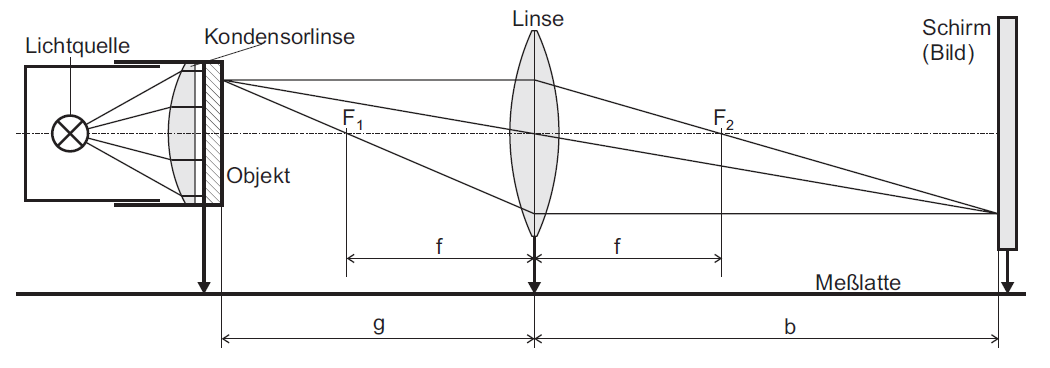
\includegraphics[width=\textwidth]{abb2}
		\captionbelowof{figure}{Schema des Aufbaues. Bildkonstruktion für einen Objektpunkt nach der geometrischen
			Optik. $g$ Gegenstandsweite, $b$ Bildweite, $f$ Brennweite.}
		\label{fig:abb2}
	\end{minipage}
\end{center}

\vspace{5mm}

\subsection{Bessel'sches Verfahren}

Hier wird der Grundsatz von der Umkehrbarkeit der Lichtwege ausgenützt. Es gelingt unter
der Voraussetzung $g + b > 4f$ für zwei Gegenstands- bzw. Bildweiten je eine reelle Abbildung
zu erhalten (\autoref{fig:abb3}). Die Brennweite steht mit der dazu notwendigen Verschiebung $e$ und dem
Gesamtabstand $g + b = a$ in folgendem Zusammenhang:

\begin{equation}
	f = \frac{1}{4} \left(\frac{a^2-e^2}{a}\right)
\end{equation}

\begin{center}
	\begin{minipage}[t]{\textwidth}
		\centering
		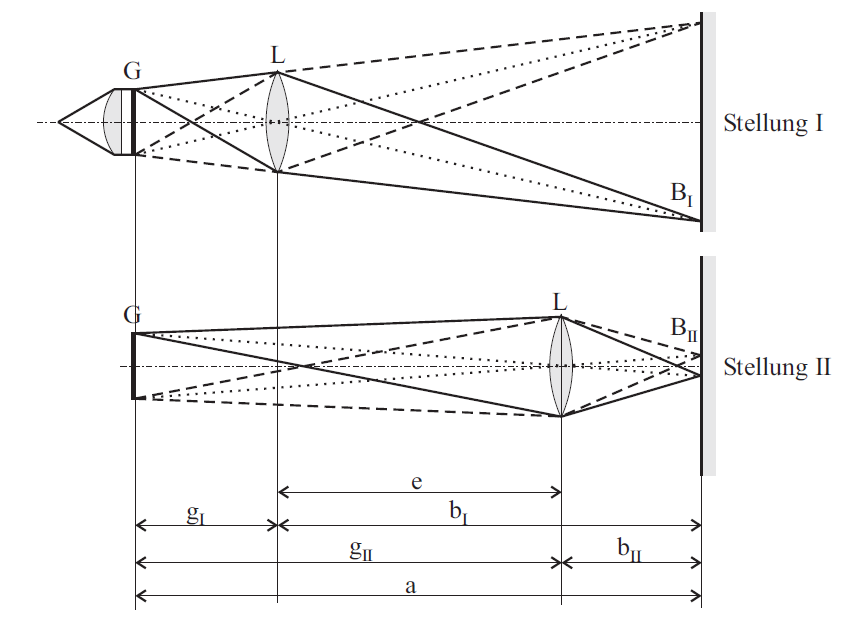
\includegraphics[width=\textwidth]{abb3}
		\captionbelowof{figure}{Die Bessel'sche Anordnung zur Messung der Brennweite. $G$ Gegenstand, $L$ Linse,
			$e$ Verschiebung, $a$ Gesamtabstand, $g_I$, $g_{II}$ Gegenstandsweiten, $b_I$, $b_{II}$ Bildweiten.}
		\label{fig:abb3}
	\end{minipage}
\end{center}

\vspace{5mm}

\subsection{Zerstreuungslinse}

\subsubsection{Methode 1}

Veränderung des Bildabstandes einer reellen Abbildung durch eine Zerstreuungslinse (\autoref{fig:abb4}).
Eine Sammellinse $L_1$ erzeugt von $G$ im Abstand $b'$ ein reelles Bild $B'$, das als
``Gegenstand``  für die Abbildung mit der nachträglich eingebrachten Zerstreuungslinse $L_2$ dient. Man erhält ganz
analog aus der Abbildungsgleichung:

\begin{equation}
	\frac{1}{f_s} = \frac{1}{g'} + \frac{1}{b}
\end{equation}

also eine negativ zu zählende Brennweite $f_2$.

\begin{center}
	\begin{minipage}[t]{\textwidth}
		\centering
		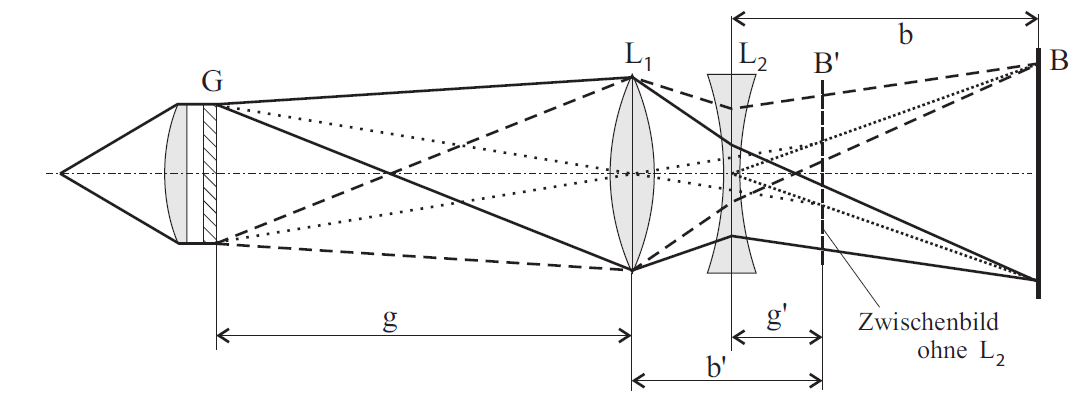
\includegraphics[width=\textwidth]{abb4}
		\captionbelowof{figure}{Kombination einer Sammelinse mit einer Zerstreuungslinse. $G$ Gegenstand, $L_1$
			Sammellinse, $L_2$ Zerstreuungslinse, $B'$ Bild mit $L_1$ ohne $L_2$, $B$ Bild mit $L_1$ und $L_2$, $g$, $g'$ Gegenstandsweite,
			$b$, $b'$ Bildweite.}
		\label{fig:abb4}
	\end{minipage}
\end{center}


\subsubsection{Methode 2}

Verändert man den Abstand der Zerstreuungslinse $L_2$ von $B'$ derart, dass $g' = -f_2$ wird (\autoref{fig:abb5}),
so rückt das Bild $B$ ins Unendliche, was mit einem auf
``unendlich`` justierten Fernrohr festgestellt
werden kann, und eine direkte Brennweitenbestimmung leicht ermöglicht.
Die Justierung des Fernrohres auf``unendlich`` erfolgt durch Anvisieren eines sehr weit entfernten
Gegenstandes hohen Kontrastes. Dies ergibt in sehr guter Näherung Unendlichstellung.

\begin{center}
	\begin{minipage}[t]{\textwidth}
		\centering
		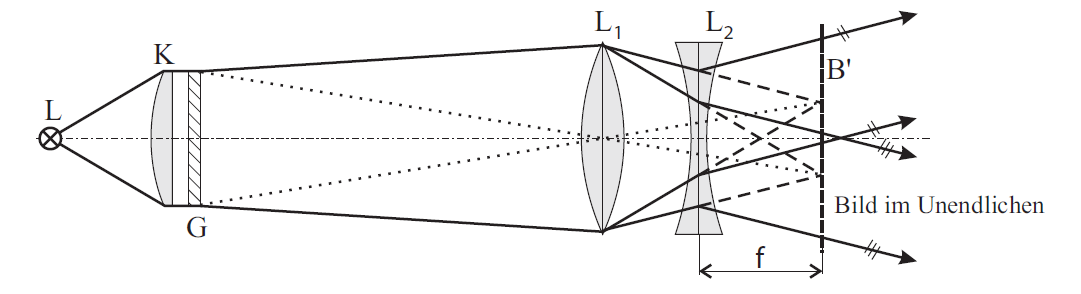
\includegraphics[width=\textwidth]{abb5}
		\captionbelowof{figure}{Kombination einer Sammellinse mit einer Zerstreuungslinse. $G$ Gegenstand, $L_1$
			Sammellinse, $L_2$ Zerstreuungslinse, $B'$ Bild nur durch Sammellinse, $B$ Bild im Unendlichen, $L$
			Lichtquelle, $K$ Kondensor, $f_2$ Brennweite der Zerstreuungslinse.}
		\label{fig:abb5}
	\end{minipage}
\end{center}


\newpage

Der tatsächliche Versuchsaufbau ist in folgender Abbildung ersichtlich.
\begin{center}
	\begin{minipage}[t]{\textwidth}
		\centering
		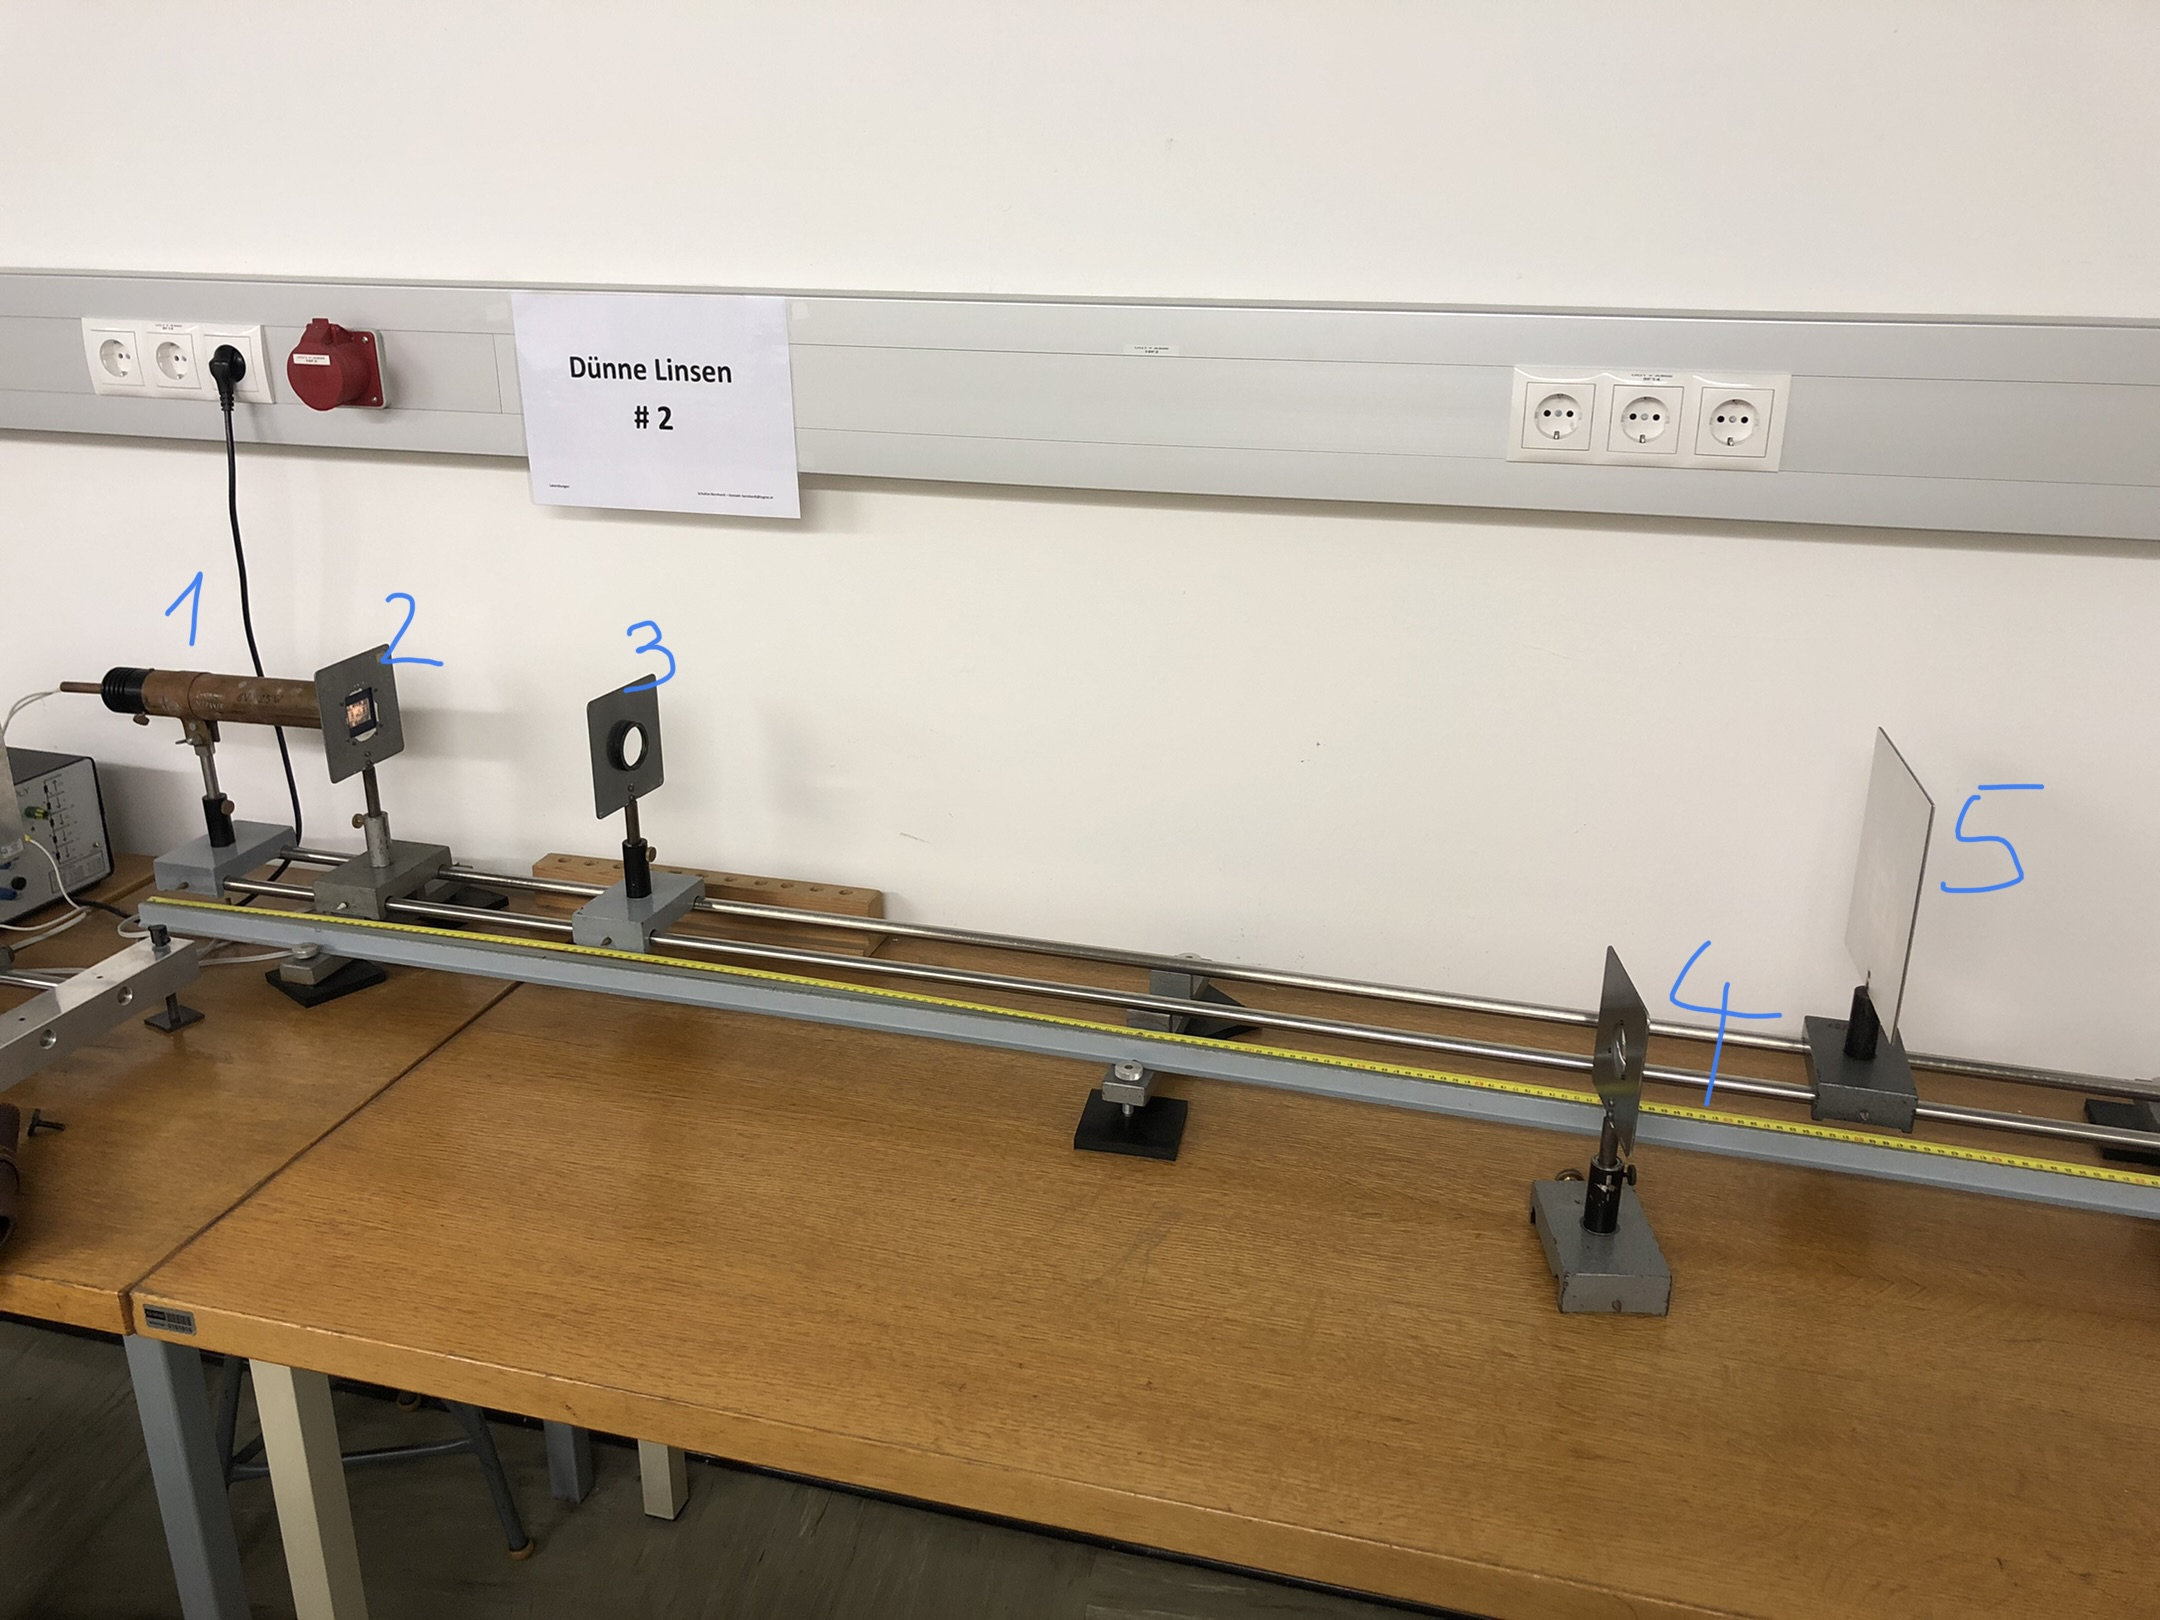
\includegraphics[width=\textwidth]{aufbau}
		\captionbelowof{figure}{Versuchsaufbau, 1 bezeichnet dabei die Lichtquelle, 2 den Gegenstand, 3 die Sammellinse, 4 die Zerstreuungslinse und 5 den Schirm}
		\label{fig:aufbau}
	\end{minipage}
\end{center}

Der Gegenstand, welcher vor die Lichtquelle geklemmt wird ist in folgender \autoref{fig:gegenstand} sichtbar.

\begin{center}
	\begin{minipage}[t]{\textwidth}
		\centering
		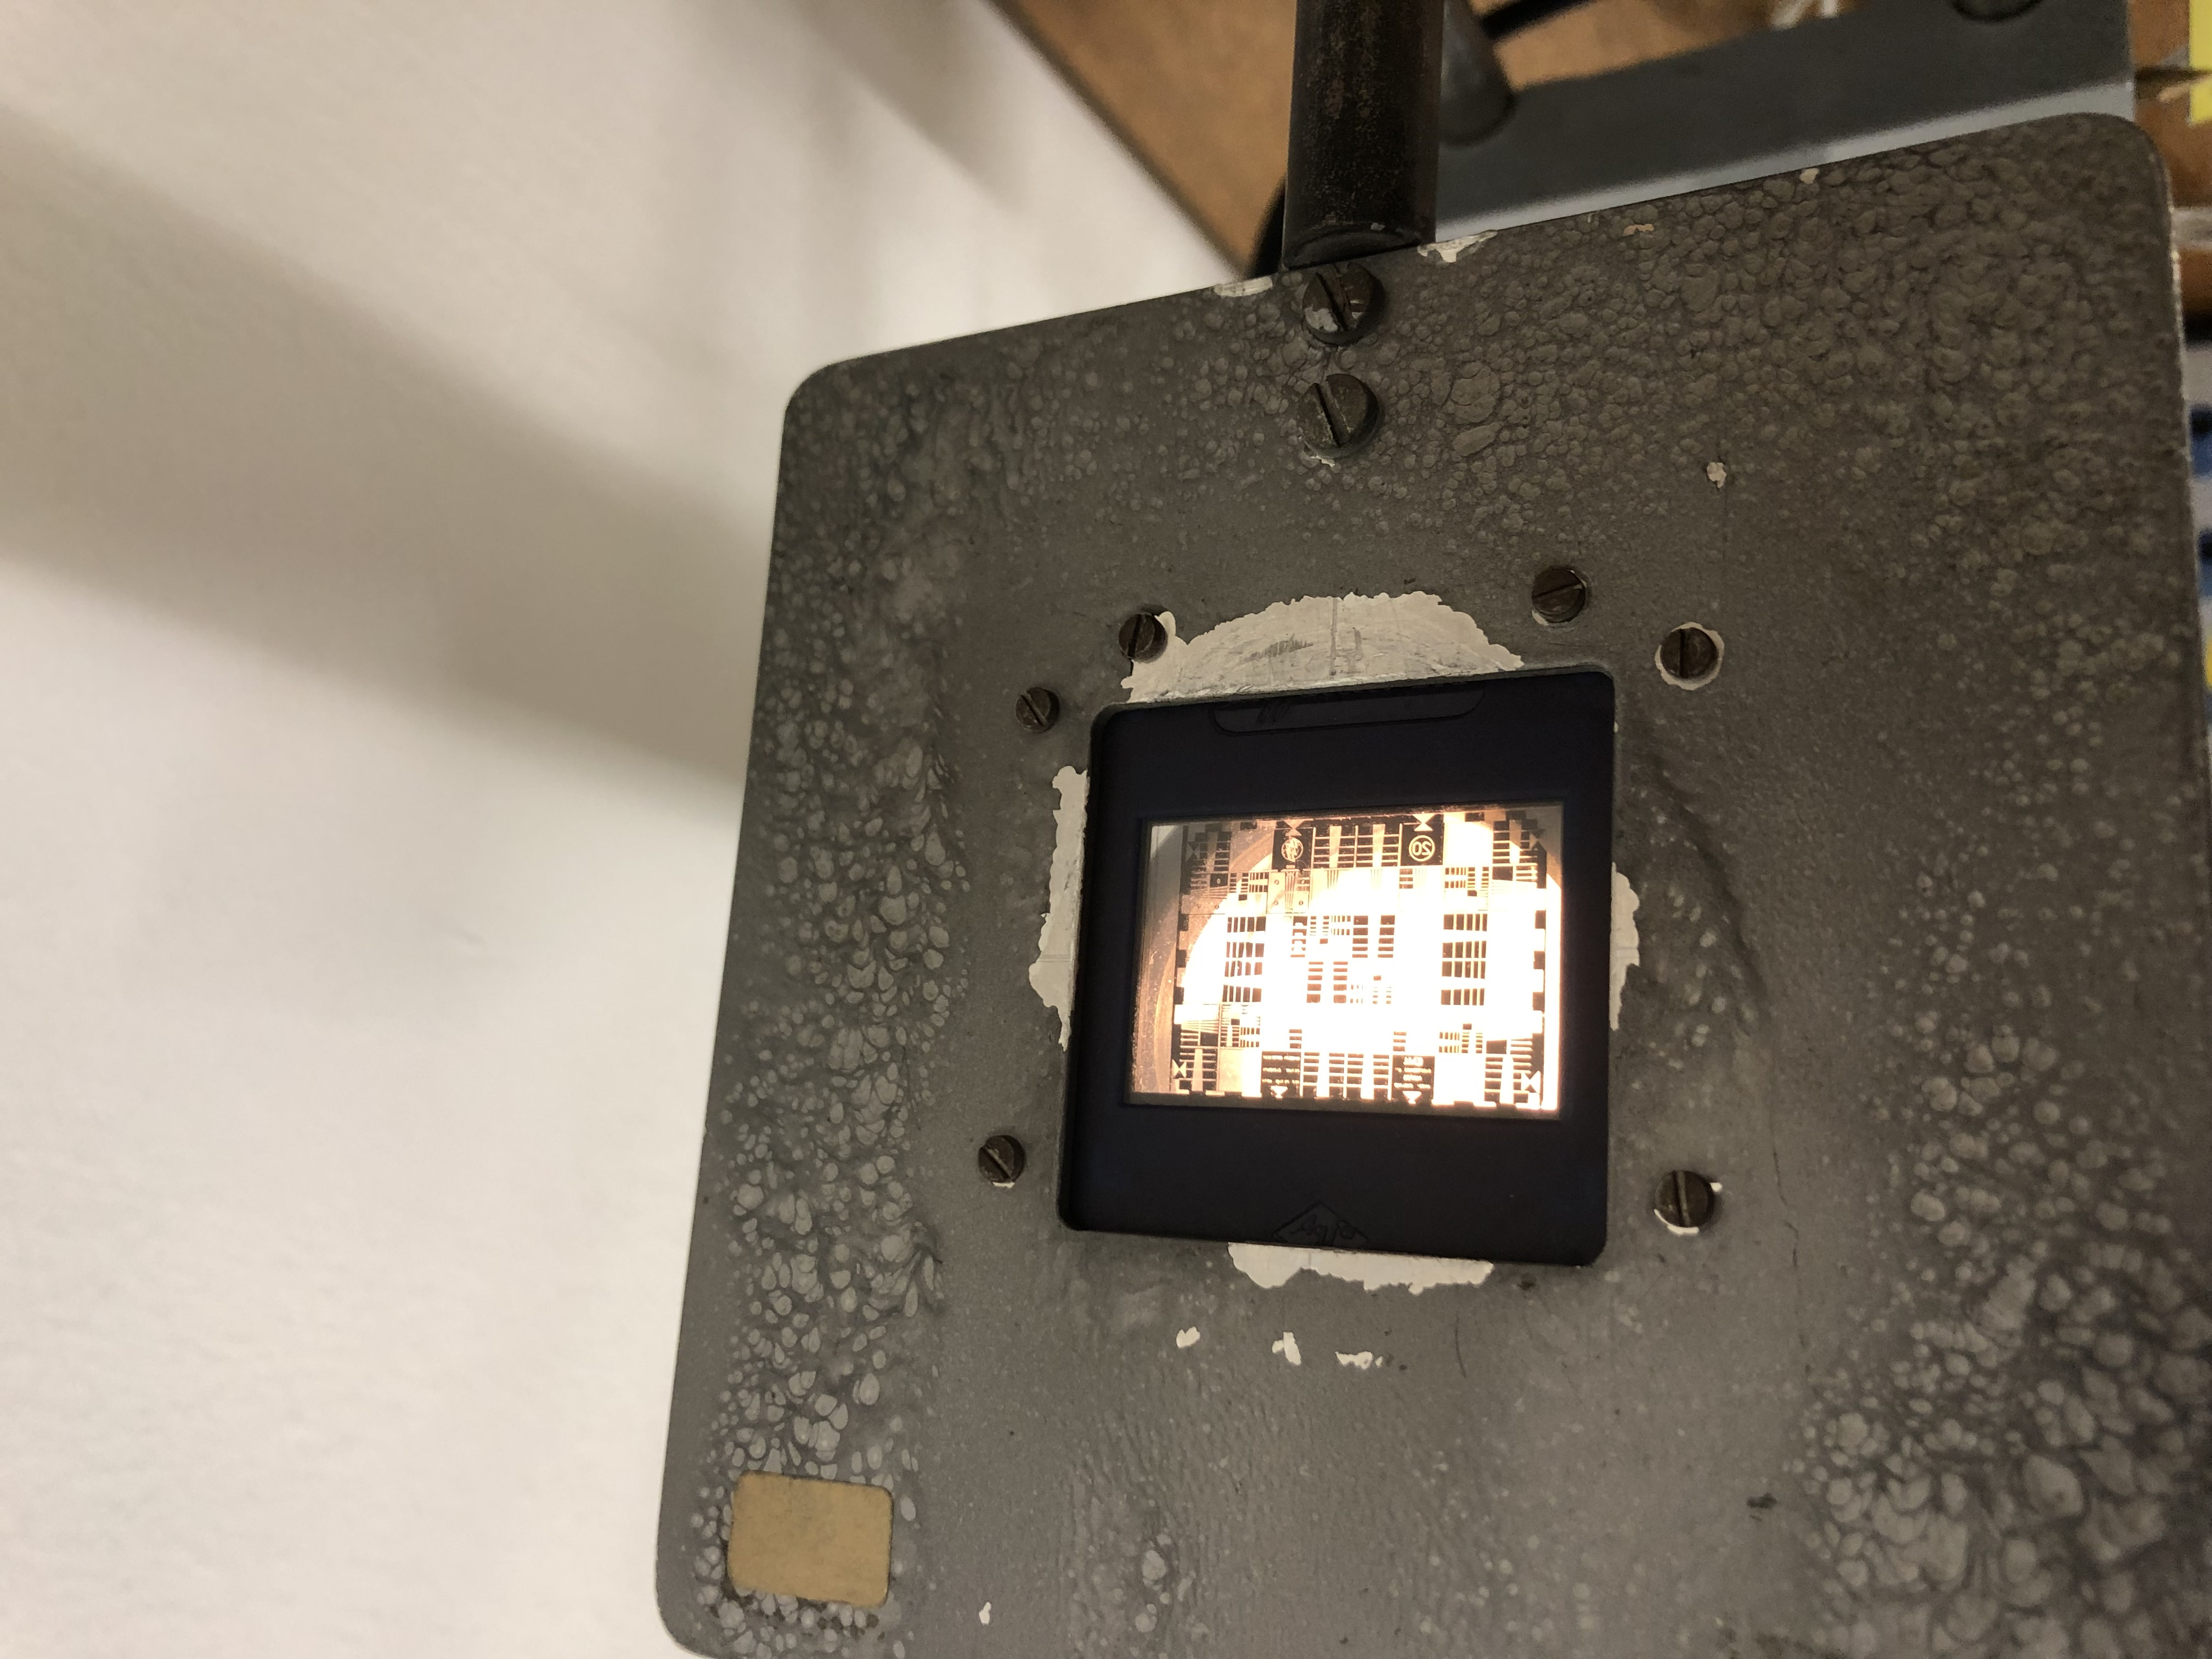
\includegraphics[angle=180,width=0.5\textwidth]{gegenstand}
		\captionbelowof{figure}{Gegenstand}
		\label{fig:gegenstand}
	\end{minipage}
\end{center}

Die Lichtquelle und der verwendete ``Power Supply`` sind in folgenden Abbildungen ersichtlich.

\vspace{2mm}

\begin{minipage}{\textwidth}
	\begin{minipage}[t]{0.5\textwidth}
		\centering
		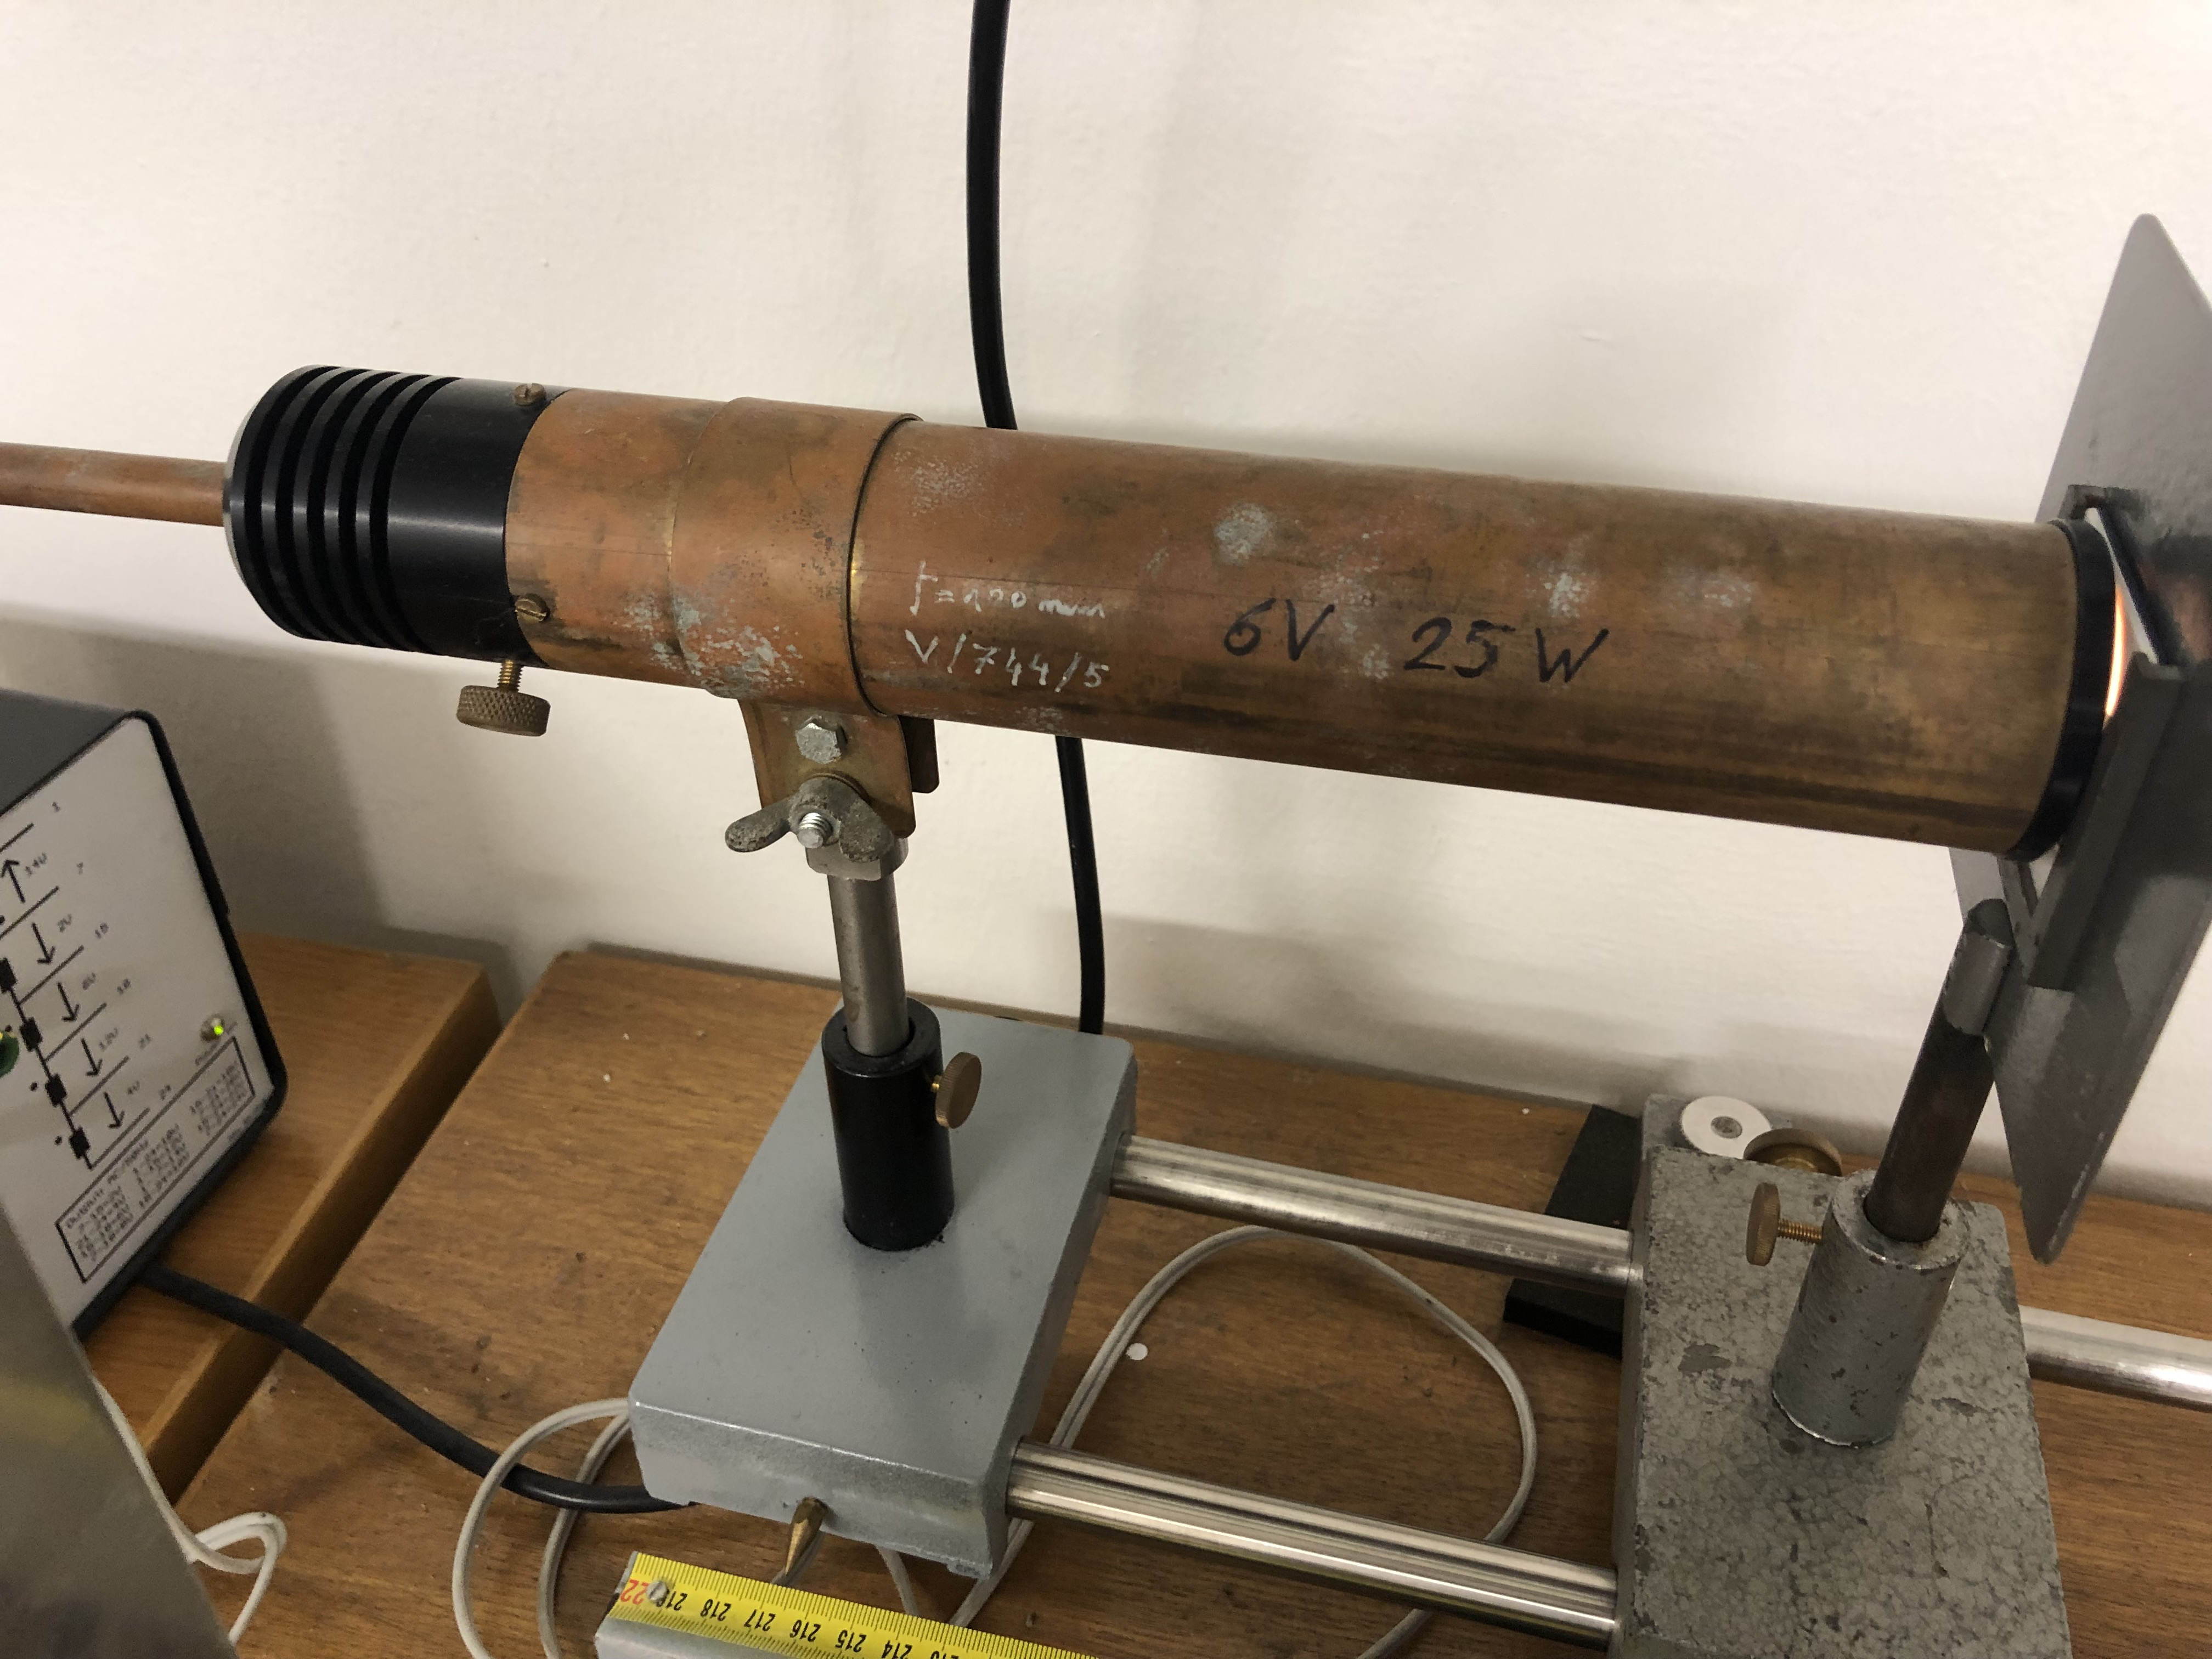
\includegraphics[width=\textwidth]{lampe}
		\captionbelowof{figure}{verwendete Lampe}
		\label{fig:lampe}
	\end{minipage}
	\vspace{2mm}
	\begin{minipage}[t]{0.50\textwidth}
		\centering
		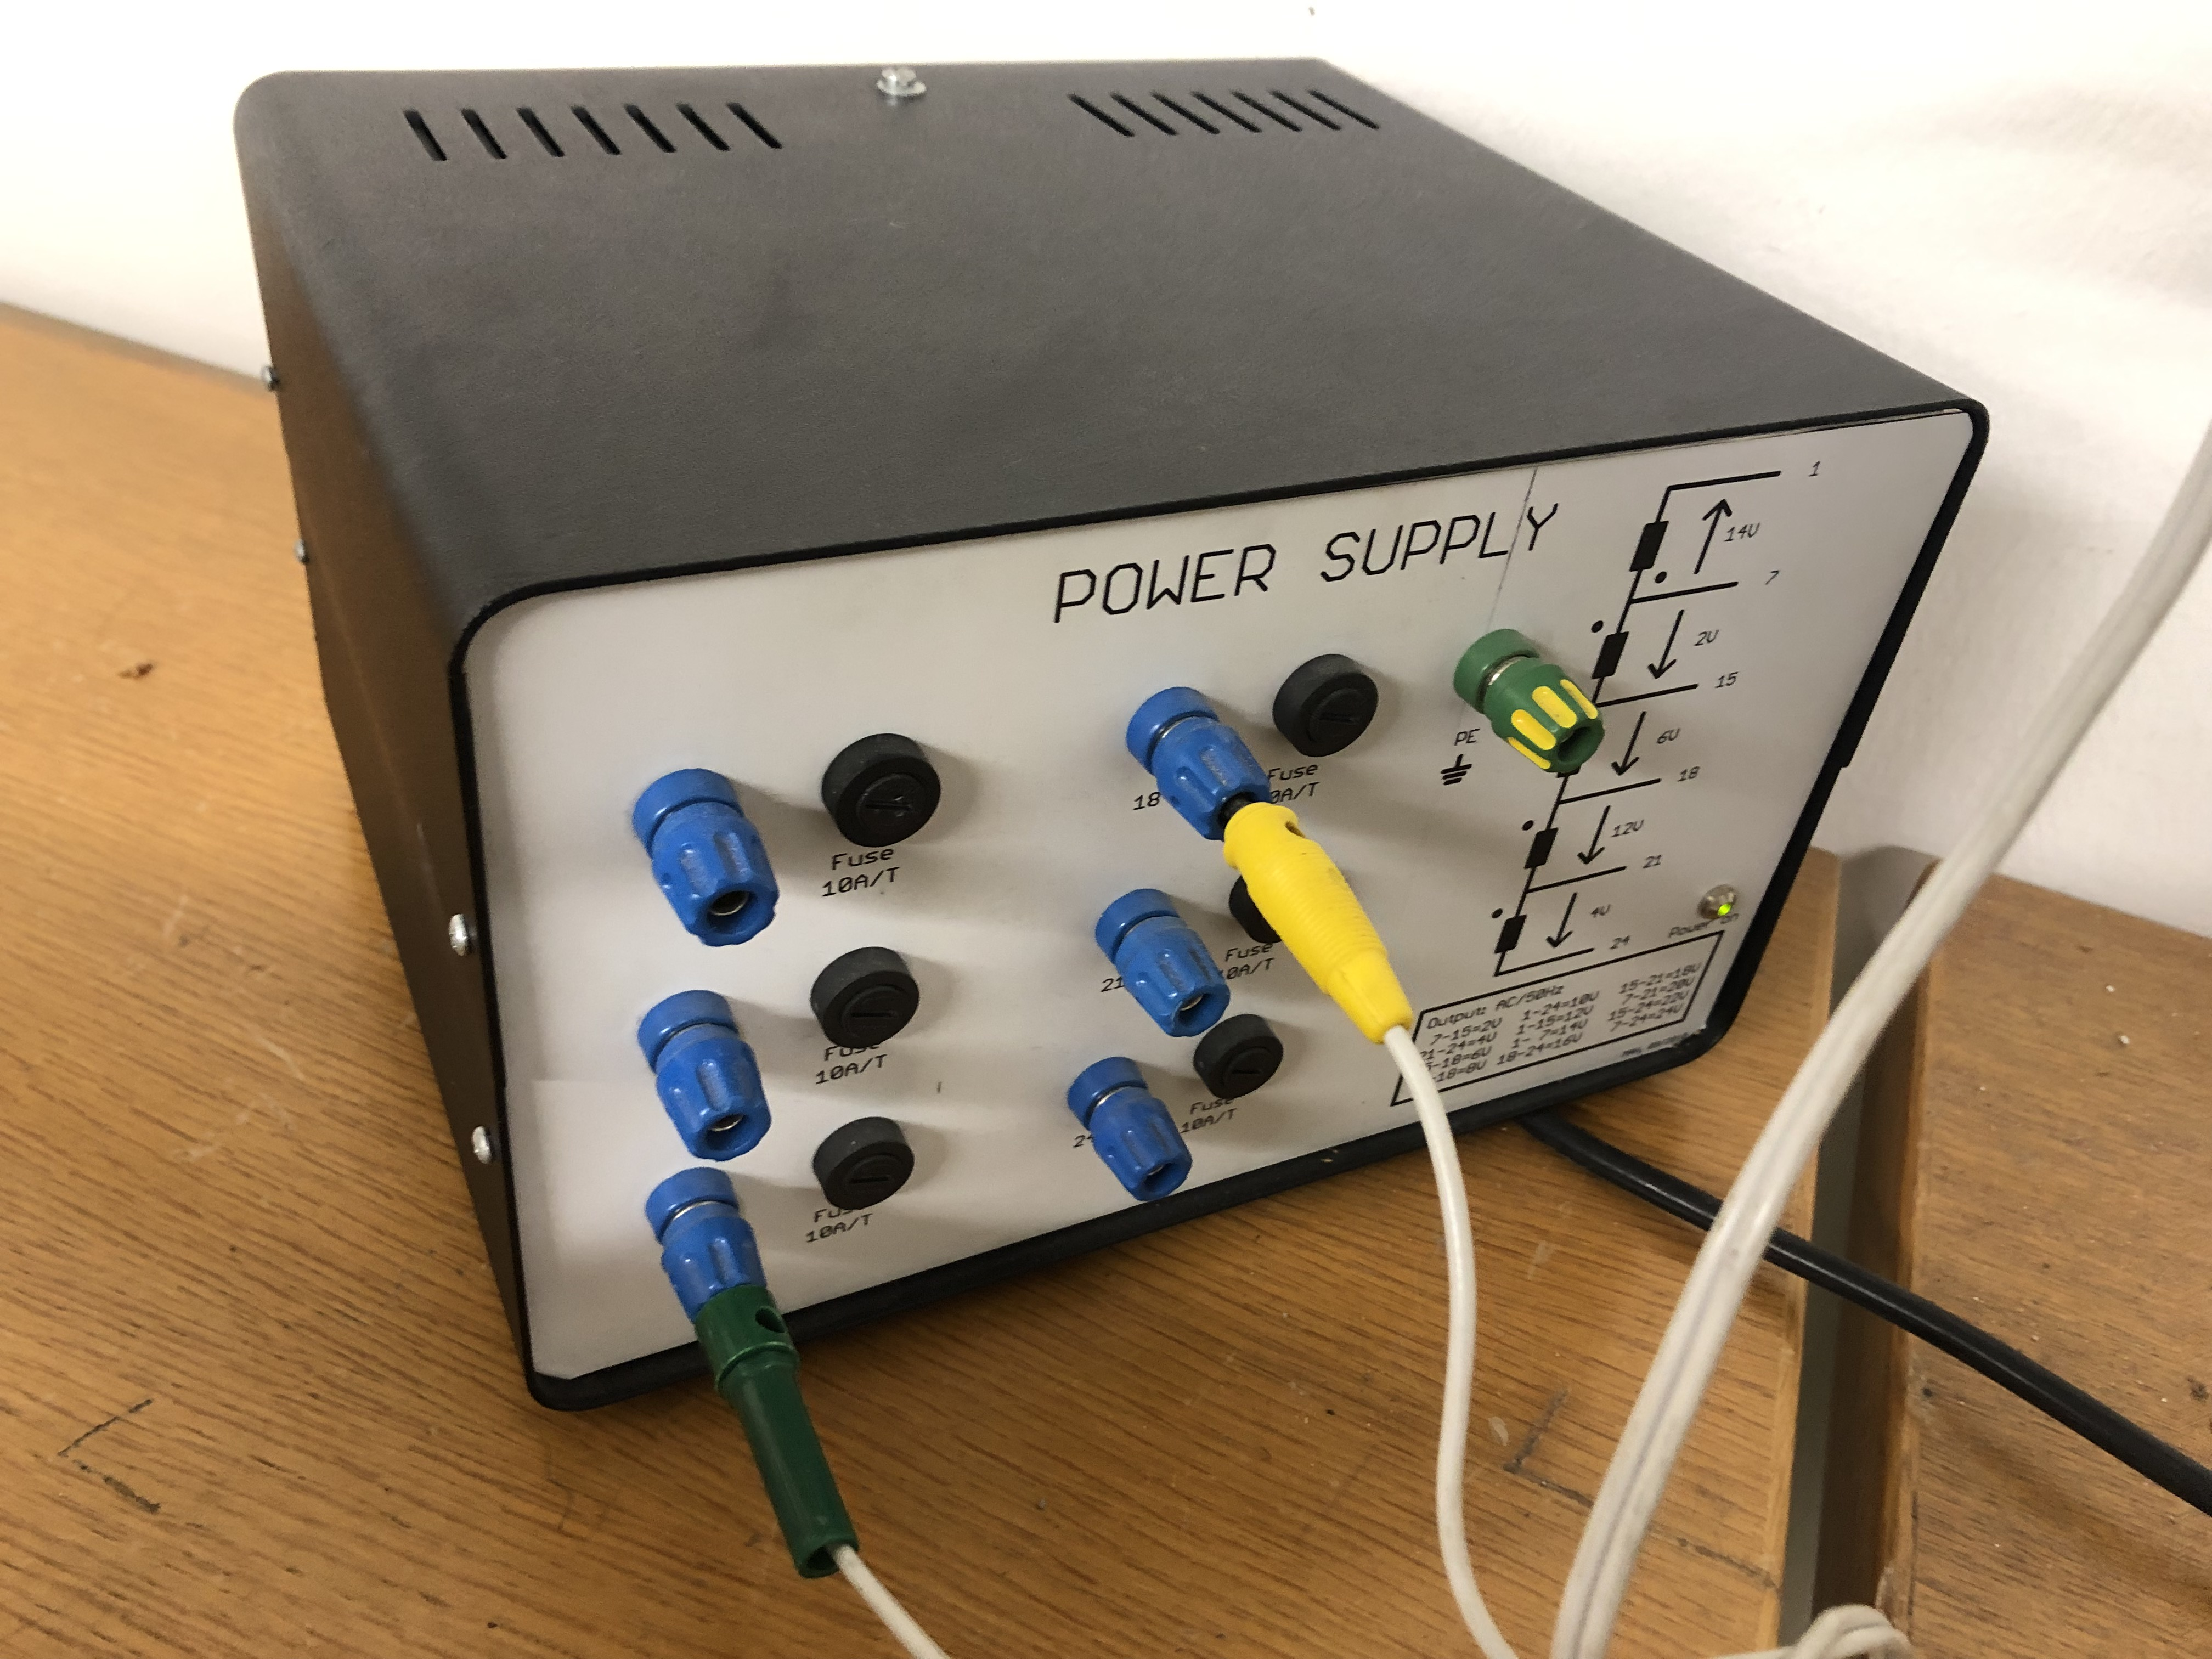
\includegraphics[width=\textwidth]{power}
		\captionof{figure}{``Power Supply``}
		\label{fig:power}
	\end{minipage}
	\vspace{1em}
\end{minipage}



\section{Geräteliste}

\noindent Für die Messungen wurden folgende Geräte verwendet:

\captionof{table}{Verwendete Geräte }
\begin{center}
	\begin{tabular}{|c|c|c|c|} \hline
		\textbf{Gerät}    & \textbf{Typ}   & \textbf{Anmerkung} \\ \hline

		Lichtquelle       & V / 744 / 5    & 6 V, 25  W         \\ \hline
		``Power Supply``  & SI 1 AT        & 230 V, 50 Az       \\ \hline
		Sammellinse       & V / 275        &                    \\ \hline
		Zerstreuungslinse & V / 275  (G20) &                    \\ \hline
		Schirm            & V / 539 / 37   &                    \\ \hline
		Gegenstand        &                &                    \\ \hline
		Optische Bank     &                &                    \\ \hline
		Maßband           &                &                    \\ \hline
	\end{tabular}
\end{center}



\section{Versuchsdurchführung \& Messergebnisse}\label{sec:Versuchsdurchführung}

Zunächst muss die optische Anordnung mithilfe eines Lasers justiert werden. Dies wurde freundlicherweise schon erledigt, sodass der Aufbau bereits justiert vorgefunden wurde. Bei der Justierung ist sicherzustellen, dass alle Linsen auf einer optischen Achse liegen.

\vspace{2mm}

Weil eine Verschiebung des Schirms schon mit bloßem Auge festgestellt werden konnte, wurde diese unter Zuhilfenahme eines Zweckentfremdeten Holzbrett, welches auf Anschlag gehalten wurde, mithilfe eines Geodreiecks der Offset des Schirm bestimmt, was einen Wert von \SI{6(2)}{mm} liefert.

Für die Unsicherheit der Linse wurde ein Wert von \SI{5}{mm} angenommen, der sich aus dessen Dicke ergibt.

Weil das Maßband nicht vollständig am Tisch befestigt war, wurde dieses mithilfe eines zusätzlichen Gewichts beschwert.

\subsection{Sammellinse}

Zunächst wird nur die Sammellinse auf der optischen Bank verwendet. Die Lichtquelle wird im gesamten Versuch nicht verschoben, weshalb die entsprechende Position des Gegenstands am Maßband abgelesen wird, was einen Wert von \SI{195.8(1)}{cm} ergibt. Um die gesamte Länge der optischen Bank zu nutzen wird der Schirm zunächst nach ganz hinten verschoben und der entsprechende Wert am Maßband abgelesen. Nun wird die Linse in der optischen Anordnung so verschoben, dass das Bild scharf am Schirm erscheint und auch diese Position ermittelt. Da dies sehr subjektiv wahrgenommen wird  wird hier besonders auf die zentralen Linien des Gegenstands, aufgrund der später erwähnten Abbildungsfehler, und die 0 geachtet. Ein scharfes Bild ist beispielhaft in \autoref{fig:bild_groß} sichtbar.

Nun wird der Schirm um \SI{10.0(1)}{cm} näher an den Gegenstand geschoben und das Bild erneut scharfgestellt. Dies wird insgesamt 10 mal wiederholt. Die so abgelesenen Werte sind in folgender Tabelle aufgelistet.

\captionof{table}{gemessene Werte \\ $L_a \dots$ gemessene Position der Lampe \\ $L \dots$ gemessene Position der Linse \\ $S \dots$ gemessene Position des Schirms \\ $L' \dots$ 2. gemessene Position der Linse für das Bessel Verfahren \\ $\Delta \dots$ entsprechende Unsicherheit}
\begin{center}
	\begin{tabular}{lrrrrrrrr}
		\toprule
		{} & $L_a$ / cm & $L$ / cm & $S$ / cm & $L'$ / cm & $\Delta L_a$ / cm & $\Delta L$ / cm & $\Delta S$ / cm & $\Delta L'$ / cm \\
		\midrule
		0  & 195.8      & 167.2    & 10.0     & 40.1      & 0.1               & 0.6             & 0.1             & 0.6              \\
		1  & 195.8      & 167.1    & 20.0     & 50.9      & 0.1               & 0.6             & 0.1             & 0.6              \\
		2  & 195.8      & 166.5    & 30.0     & 61.4      & 0.1               & 0.6             & 0.1             & 0.6              \\
		3  & 195.8      & 165.9    & 40.0     & 72.6      & 0.1               & 0.6             & 0.1             & 0.6              \\
		4  & 195.8      & 165.1    & 50.0     & 83.1      & 0.1               & 0.6             & 0.1             & 0.6              \\
		5  & 195.8      & 164.0    & 60.0     & 94.1      & 0.1               & 0.6             & 0.1             & 0.6              \\
		6  & 195.8      & 162.6    & 70.0     & 105.3     & 0.1               & 0.6             & 0.1             & 0.6              \\
		7  & 195.8      & 161.0    & 80.0     & 117.1     & 0.1               & 0.6             & 0.1             & 0.6              \\
		8  & 195.8      & 157.4    & 90.0     & 131.2     & 0.1               & 0.6             & 0.1             & 0.6              \\
		9  & 195.8      & 151.0    & 100.0    & 151.0     & 0.1               & 0.6             & 0.1             & 0.6              \\
		\bottomrule
	\end{tabular}
	\label{tab:werte_sammellinse}
\end{center}

Um die Brennweite nach dem Bessel´schen verfahren bestimmen zu könne, muss ein zweites kleineres scharfes Bild durch eine andere Position der Linse erzeugt werden, wie in \autoref{fig:bild_klein} ersichtlich. Die entschiedene Größe ist dabei die Differenz zwischen den beiden Positionen, an denen der Gegenstand scharf erscheint. Weil die erste Position der Linse den bereits zuvor bestimmten Werten entspricht, wird die zweite Position der Linse gleich im Zuge des ersten Versuchs mitbestimmt, was in obiger \autoref{tab:werte_sammellinse} bereits hinzugefügt wurde. Dabei ist anzumerken, dass die Distanz zwischen den beiden Linsenpunkten vor allem bei einem nahen Schirm immer kleiner wurde, wobei bei der letzten Messung gar nicht mehr zwischen den Positionen unterschieden werden konnte.

\vspace{2mm}

\begin{minipage}{\textwidth}
	\begin{minipage}[t]{0.5\textwidth}
		\centering
		\includegraphics[width=\textwidth]{bild_groß}
		\captionbelowof{figure}{sichtbares Bild des Gegenstands}
		\label{fig:bild_groß}
	\end{minipage}
	\vspace{2mm}
	\begin{minipage}[t]{0.50\textwidth}
		\centering
		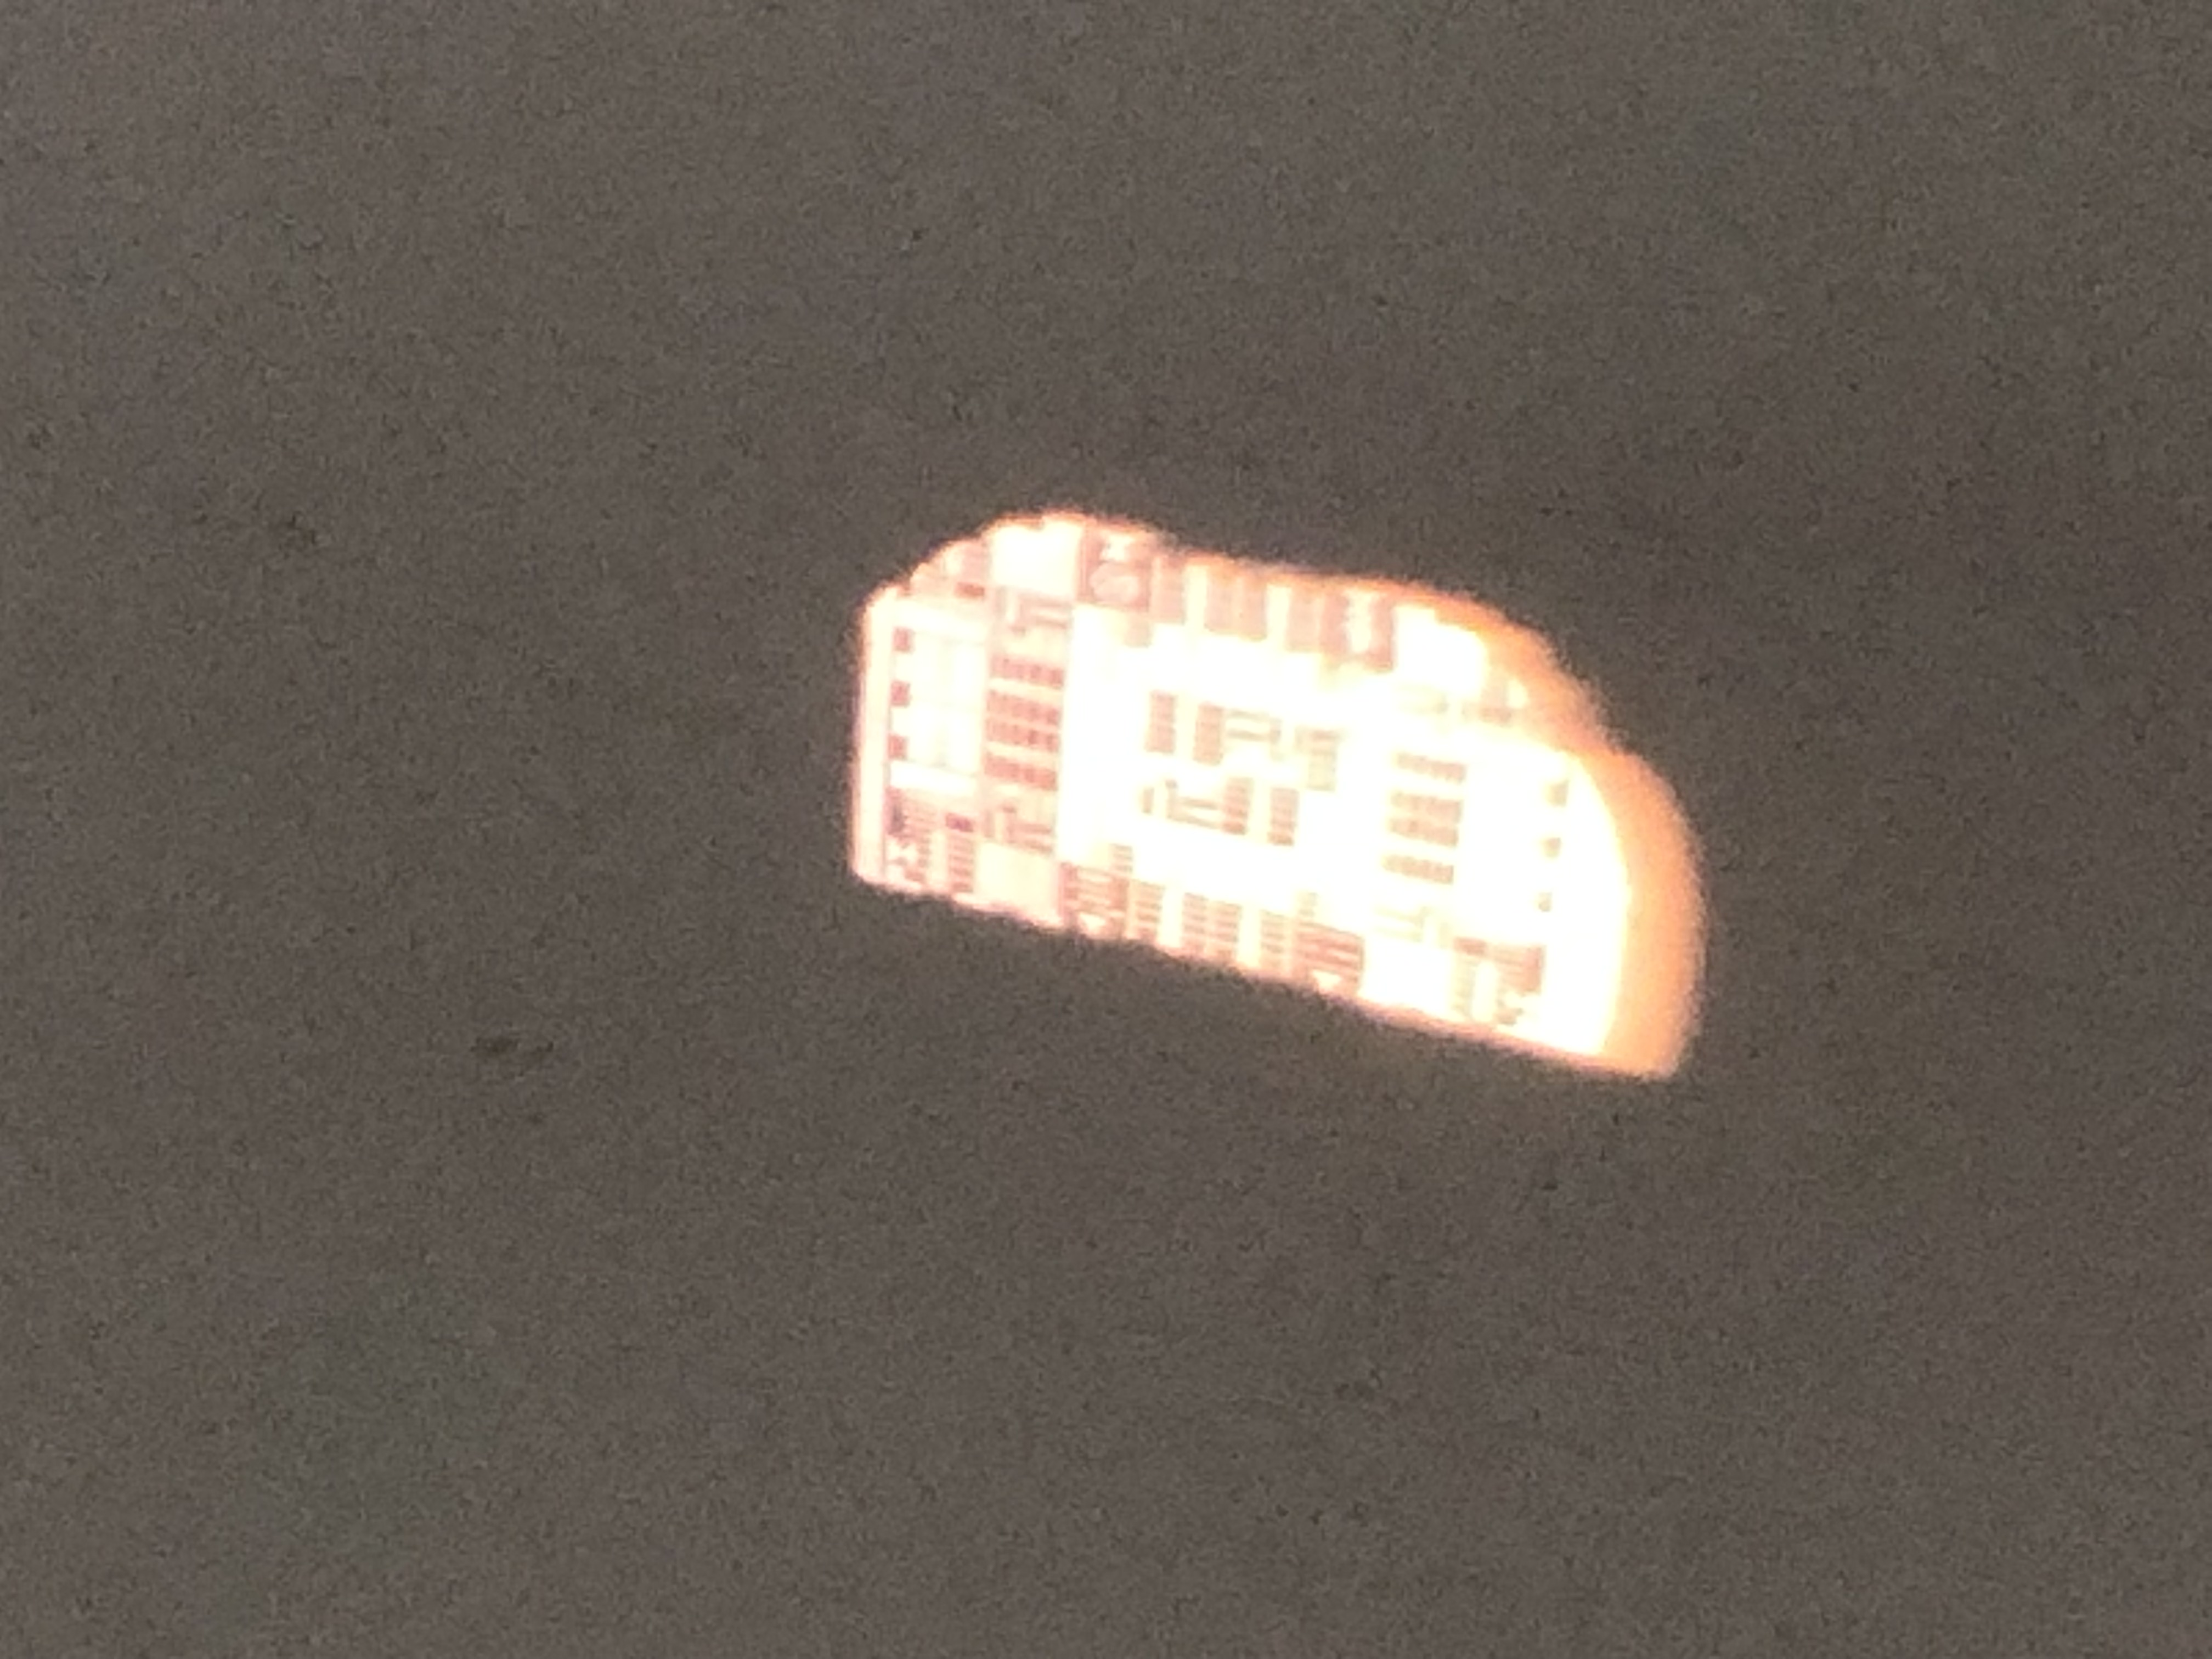
\includegraphics[width=\textwidth]{bild_klein}
		\captionof{figure}{kleines Bild des Gegenstands für den ``Bessel-aufbau``}
		\label{fig:bild_klein}
	\end{minipage}
	\vspace{1em}
\end{minipage}


\subsection{Zerstreuungslinse}

Um die Brennweite der Zerstreuungslinse zu bestimmen, wird zunächst die Sammellinse in die Mitte der optischen Bank, auf die Position von \SI{100.0(1)}{cm} geschoben und mithilfe der Schirms die Position des entsprechenden Bild bestimmt, was im konkreten Fall einen Wert von \SI{65.4(1)}{cm} entspricht. Nun wird die Zerstreuungslinse in den Strahlengang gestellt und mithilfe des Schirms die Position des neuen Bilds bestimmt. Wichtig dabei ist, dass die Sammellinse nicht mehr verschoben wird. Dieser Vorgang wird für 10 verschiedene Positionen der Zerstreuungslinse wiederholt, was folgende Werte liefert.

\captionof{table}{gemessene Werte \\ $S \dots$ gemessene Position des Schirms \\ $L_z \dots$ gemessene Position der Zerstreuungslinse \\ $\Delta \dots$ entsprechende Unsicherheit}
\begin{center}
	\begin{tabular}{lrrrr}
		\toprule
		{} & $S$ / cm & $L_{z}$ / cm & $\Delta S$ / cm & $\Delta L_{z}$ / cm \\
		\midrule
		0  & 4.0      & 78.0         & 0.1             & 0.5                 \\
		1  & 29.4     & 77.0         & 0.1             & 0.5                 \\
		2  & 42.1     & 76.0         & 0.1             & 0.5                 \\
		3  & 50.3     & 75.0         & 0.1             & 0.5                 \\
		4  & 55.2     & 74.0         & 0.1             & 0.5                 \\
		5  & 57.9     & 73.0         & 0.1             & 0.5                 \\
		6  & 37.2     & 76.5         & 0.1             & 0.5                 \\
		7  & 45.4     & 75.5         & 0.1             & 0.5                 \\
		8  & 53.4     & 74.5         & 0.1             & 0.5                 \\
		9  & 56.4     & 73.5         & 0.1             & 0.5                 \\
		\bottomrule
	\end{tabular}
	\label{tab:werte_zerstreuungslinse}
\end{center}

Weil der Aufbau mit dem im unendlichen fokussierten Fernrohr mit den zur Verfügung stehenden Mitteln leider nicht gut durchführbar ist, wurde dieser unter Absprache mit dem Betreuer weggelassen.

\vspace{5mm}

\section{Auswertung}

\noindent Um zu sehen wie sich die Unsicherheit der Messungen bis in die Ergebnisse
fortplanzt, ist \autoref{eq:Unsicherheitsfortpflanzung} verwendet worden.
Die Grundlagen dieser Gleichung stammen von den Powerpointfolien von
GUM.\cite{WolfgangKessel2004} Die Verallgemeinerung ist von Wikipedia entnommen
worden \cite{2020Fehler}.
Für die Auswertung ist die Progammiersprache Python im speziellen das
Packet \verb#scipy#, zur Hilfe genommen worden.

\begin{equation}
	\label{eq:Unsicherheitsfortpflanzung}
	V_y = J(\bm{x}) \cdot V_x \cdot J^{T}(\bm{x})
\end{equation}

\noindent Wobei $V_y$ und $V_x$ die Kovarianzmatrizen von den Vektoren $\bm{y}$ und $\bm{x}$ sind.
$\bm{x}$ ist der Vektor der Eingangsvariablen und $\bm{y}$ ist der Vektor der Ausgangsvariablen.
$J$ ist die Jakobimatrix der vektorwertigen Funktion $\bm{y} = \vec{F}(\bm{x})$.
So lassen sich die Komponenten der Matrix relativ einfach anschreiben $J_{ij}(x) = \frac{\partial{y_i}}{\partial{x_j}}(x)$.
Damit man die Unsicherheit der einzelnen Variablen $y_i$ bekommt, muss nur die Quadratwurzel des i-ten Diagonalelementes der
$\bm{y}$-Kovarianzmatrix genommen werden $u_i= \sqrt{\mathrm{diag}(V_y)_i}$.
Da in diesem Experiment meistens nur skalare Funktionen untersucht werden, vereinfacht
sich die \autoref{eq:Unsicherheitsfortpflanzung} dramatisch und die Unsicherheit
der Variable $y$ lässt sich einfach so berechnen:

\begin{equation}
	\label{eq:graduncentainty}
	u_y = \sqrt{\mathrm{grad} y^T \cdot V_x \cdot \mathrm{grad} y}
\end{equation}


\vspace{2mm}

Bei den Messwerten ist angenommen worden, dass diese normalverteilt gemessen
werden, weshalb bei der Mittelwertbildung der Student t Korrekturfaktor für ein
3 $\sigma$ Intervall bei 10 Messwerten genommen wurde.

\begin{align*}
	t = 4.09
\end{align*}

\newpage

\subsection{Sammellinse}

\subsubsection{Laplace´sche Methode}

Zunächst werden anhand der gemessenen Daten aus \autoref{tab:werte_sammellinse} die gesuchten Distanzen bestimmt, was in folgender Tabelle sichtbar ist. Dabei ist auch der Offset des Schirms zu berücksichtigen.

\captionof{table}{gemessene Werte \\ $b \dots$ errechnete Distanz für die Bildweite \\ $g \dots$ errechnete Distanz für die Gegenstandsweite \\ $\Delta \dots$ entsprechende Unsicherheit}
\begin{center}
	\begin{tabular}{lrrrr}
		\toprule
		{} & $b$ / cm & $g$ / cm & $\Delta b$ / cm & $\Delta g$ / cm \\
		\midrule
		0  & 156.6    & 28.6     & 0.9             & 0.7             \\
		1  & 146.5    & 28.7     & 0.9             & 0.7             \\
		2  & 135.9    & 29.3     & 0.9             & 0.7             \\
		3  & 125.3    & 29.9     & 0.9             & 0.7             \\
		4  & 114.5    & 30.7     & 0.9             & 0.7             \\
		5  & 103.4    & 31.8     & 0.9             & 0.7             \\
		6  & 92.0     & 33.2     & 0.9             & 0.7             \\
		7  & 80.4     & 34.8     & 0.9             & 0.7             \\
		8  & 66.8     & 38.4     & 0.9             & 0.7             \\
		9  & 50.4     & 44.8     & 0.9             & 0.7             \\
		\bottomrule
	\end{tabular}
\end{center}

Nun werden anhand dieser Werte und Gleichung 1 wie Werte für die Brennweiten bestimmt, was in folgender Tabelle sichtbar ist.

\captionof{table}{gemessene Werte \\ $f \dots$ errechnete Werte für die Brennweiten der Sammellinse nach der Laplace´schen Methode\\ $\Delta \dots$ entsprechende Unsicherheit}
\begin{center}
	\begin{tabular}{lrr}
		\toprule
		{} & $f$ / cm & $\Delta f$ / cm \\
		\midrule
		0  & 24.2     & 0.6             \\
		1  & 24.0     & 0.6             \\
		2  & 24.1     & 0.6             \\
		3  & 24.1     & 0.5             \\
		4  & 24.2     & 0.5             \\
		5  & 24.3     & 0.5             \\
		6  & 24.4     & 0.5             \\
		7  & 24.3     & 0.5             \\
		8  & 24.4     & 0.5             \\
		9  & 23.7     & 0.4             \\
		\bottomrule
	\end{tabular}
\end{center}

Bildet man daraus den Mittelwert, so ergibt sich \SI{24.2(8)}{\cm}.

\newpage

Die Werte werden auch in folgende Grafik eingezeichnet, wodurch die Brennweite anhand der Fitgeraden bestimmt werden kann.

\begin{center}
	\begin{minipage}[t]{\textwidth}
		\centering
		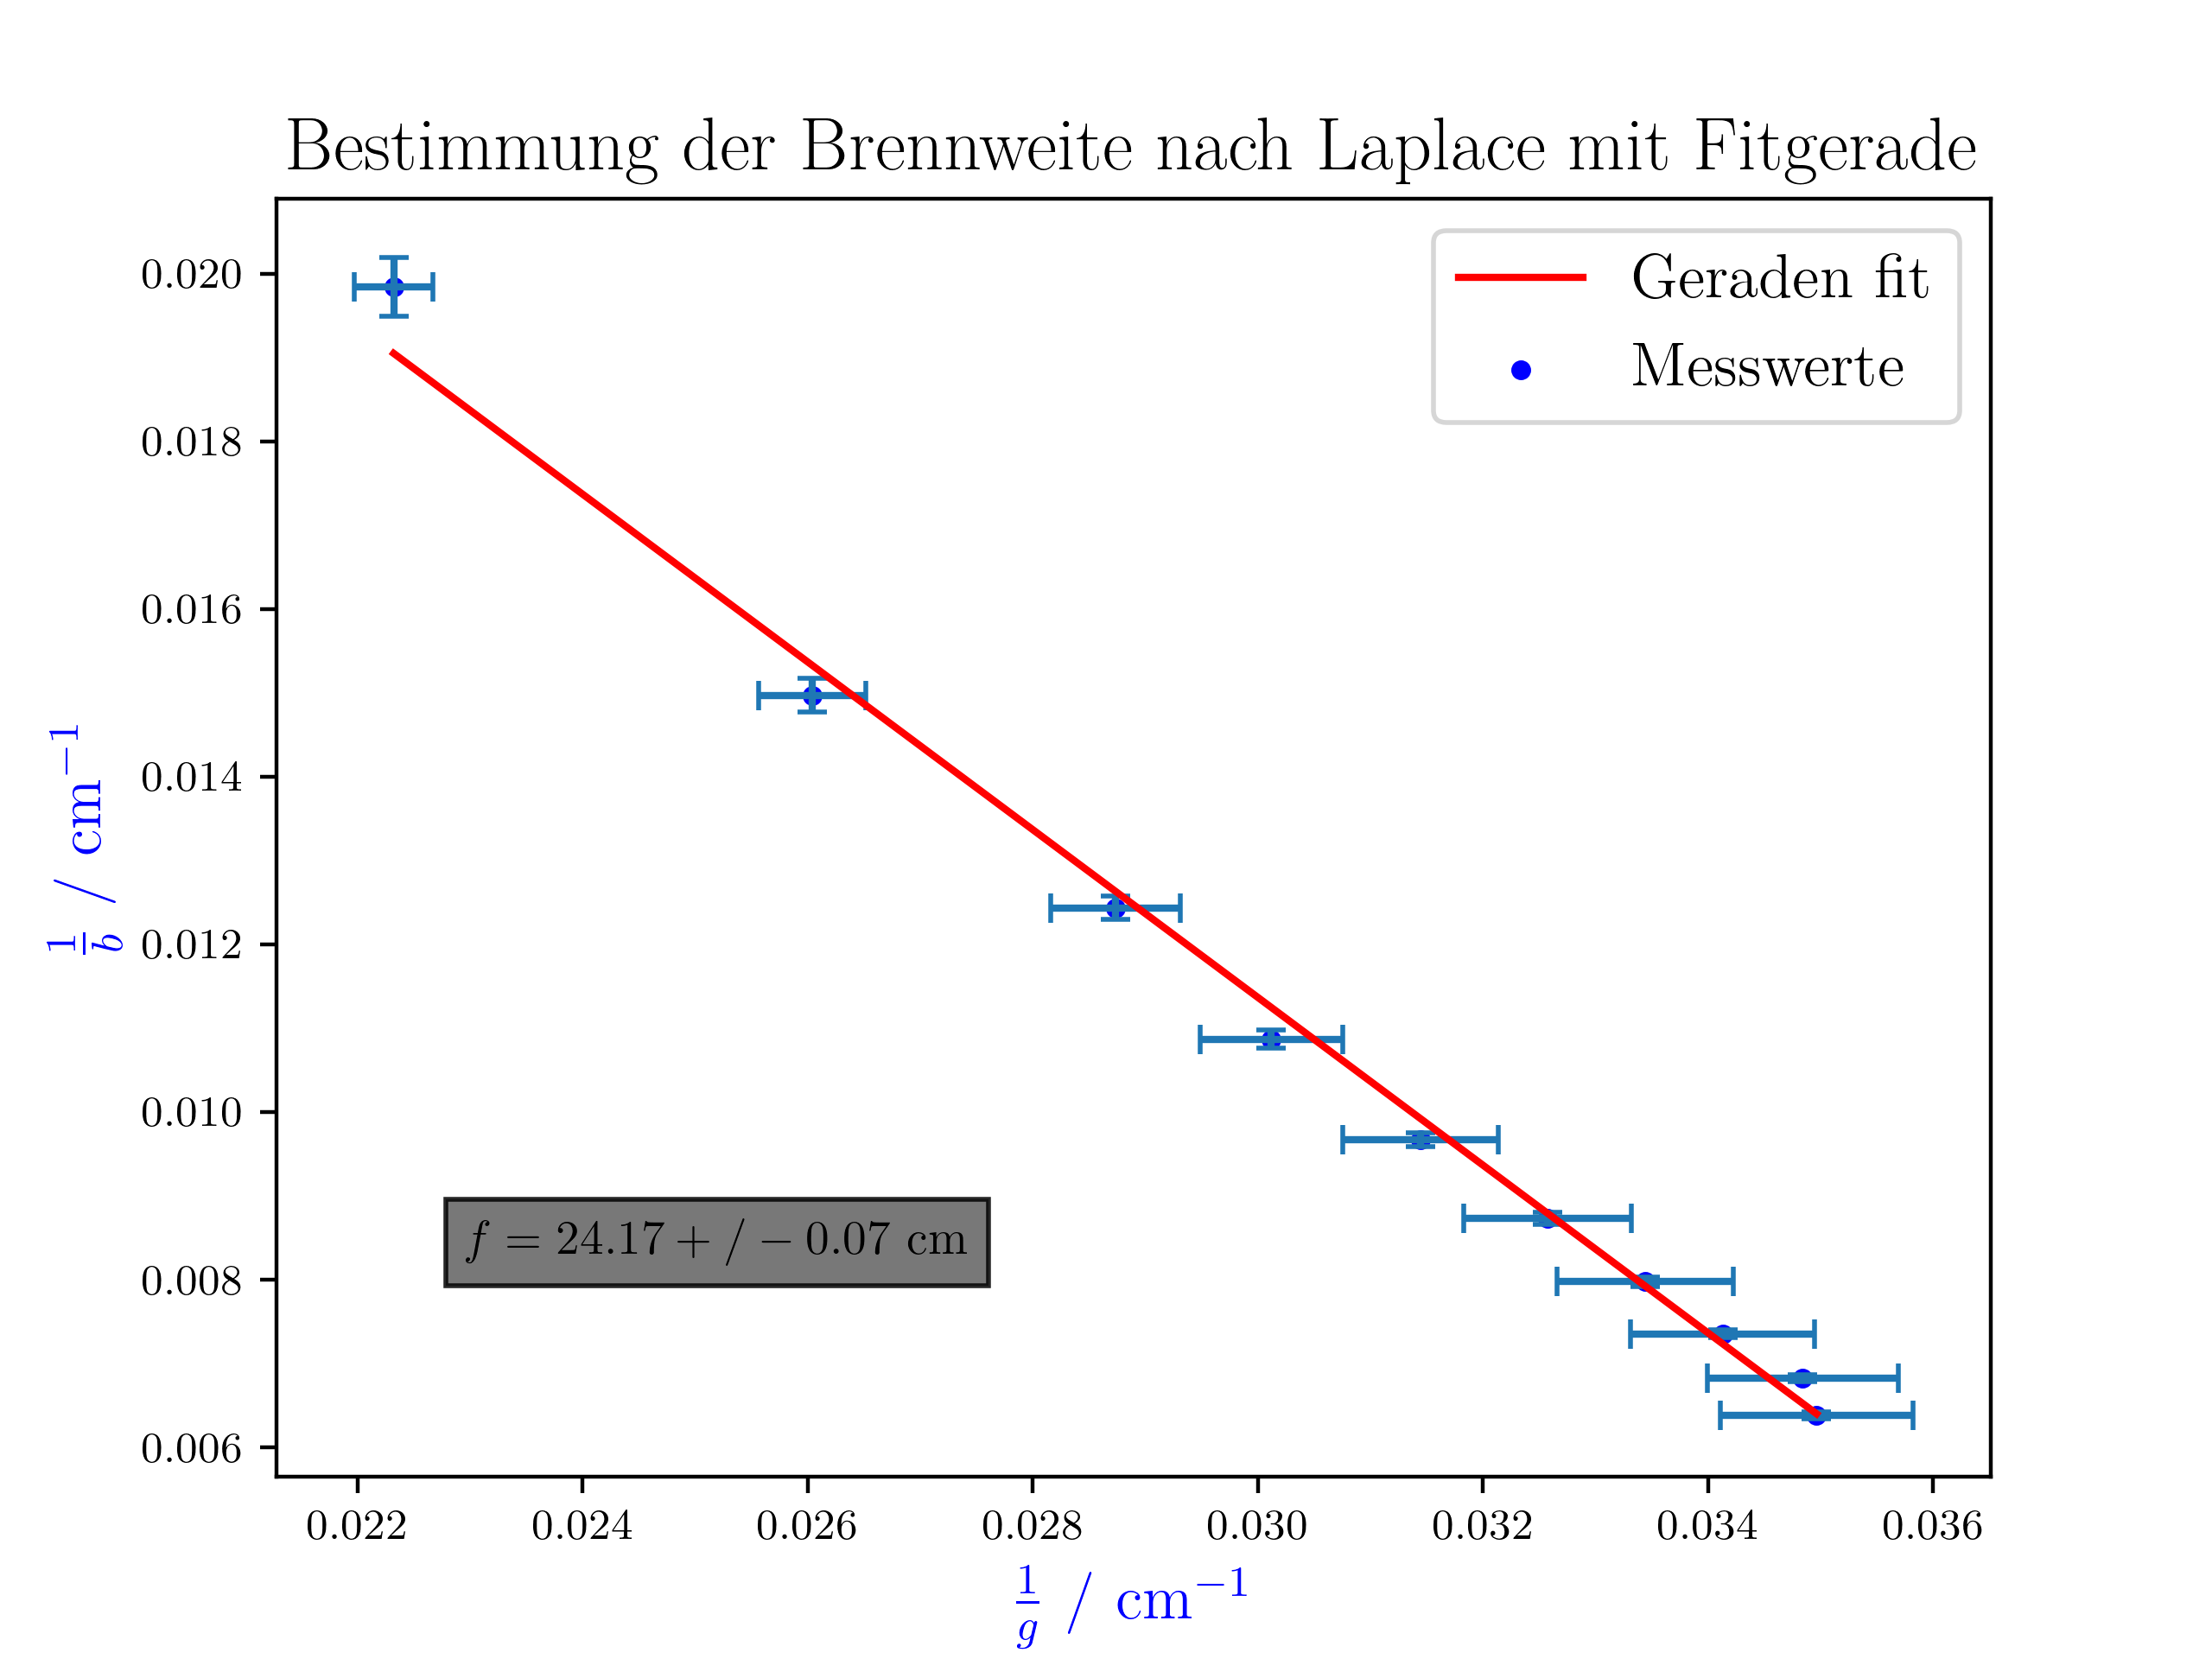
\includegraphics[width=0.8\textwidth]{fit}
		\captionbelowof{figure}{Bestimmung der Brennweite nach der Laplace Methode mit Fitgeraden}
		\label{fig:fit}
	\end{minipage}
\end{center}

Auch daraus ergibt sich wieder der selbe Wert für die gemittelte Brennweite.

\newpage

\subsubsection{Bessel´sche Methode}

Anhand der Daten aus \autoref{tab:werte_sammellinse} werden nun die Werte für die entsprechenden Daten bestimmt, was in folgender Tabelle sichtbar ist. Auch hier ist wieder der Offset des Schirms zu berücksichtigen.

\captionof{table}{gemessene Werte \\ $a \dots$ errechnete Distanz für den Gesamtabstand \\ $e \dots$ errechnete Distanz für die Verschiebung \\ $\Delta \dots$ entsprechende Unsicherheit}
\begin{center}
	\begin{tabular}{lrrrr}
		\toprule
		{} & $a$   & $\Delta a$ & $e$   & $\Delta e$ \\
		\midrule
		0  & 186.4 & 0.4        & 127.1 & 1.2        \\
		1  & 176.4 & 0.4        & 116.2 & 1.2        \\
		2  & 166.4 & 0.4        & 105.1 & 1.2        \\
		3  & 156.4 & 0.4        & 93.3  & 1.2        \\
		4  & 146.4 & 0.4        & 82.0  & 1.2        \\
		5  & 136.4 & 0.4        & 69.9  & 1.2        \\
		6  & 126.4 & 0.4        & 57.3  & 1.2        \\
		7  & 116.4 & 0.4        & 43.9  & 1.2        \\
		8  & 106.4 & 0.4        & 26.2  & 1.2        \\
		9  & 96.4  & 0.4        & 0.0   & 1.2        \\
		\bottomrule
	\end{tabular}
\end{center}

Verwendet man diese Werte zusammen mit Formel 2 erhält man für die Brennweiten folgende Werte.

\captionof{table}{gemessene Werte \\ $f \dots$ errechnete Werte für die Brennweiten der Sammellinse nach der Bessel´schen Methode\\ $\Delta \dots$ entsprechende Unsicherheit}
\begin{center}
	\begin{tabular}{lrr}
		\toprule
		{} & $f$ / cm & $\Delta f$ / cm \\
		\midrule
		0  & 24.9     & 0.5             \\
		1  & 25.0     & 0.5             \\
		2  & 25.0     & 0.4             \\
		3  & 25.2     & 0.4             \\
		4  & 25.1     & 0.4             \\
		5  & 25.1     & 0.4             \\
		6  & 25.1     & 0.3             \\
		7  & 25.0     & 0.3             \\
		8  & 25.0     & 0.2             \\
		9  & 24.10    & 0.05            \\
		\bottomrule
	\end{tabular}
\end{center}

Bildet man daraus den Mittelwert, so ergibt sich \SI{25.0(13)}{\cm}.

\newpage

\subsection{Zerstreuungslinse}

Zunächst werden die Werte aus \autoref{tab:werte_zerstreuungslinse} verwendet und die Werte für die Parameter für $b$ und $g'$ zu bestimmen, was folgende Werte liefert.

\captionof{table}{gemessene Werte \\ $b \dots$ errechnete Distanz für die Bildweite nach der Zerstreuungslinse \\ $g' \dots$ errechnete Distanz für die Gegenstandsweite der Zerstreuungslinse \\ $\Delta \dots$ entsprechende Unsicherheit}
\begin{center}
	\begin{tabular}{lrrrr}
		\toprule
		{} & $b$ / cm & $g'$ / cm & $\Delta b$ / cm & $\Delta g'$ / cm \\
		\midrule
		0  & 73.4     & -12.0     & 0.8             & 0.8              \\
		1  & 47.0     & -11.0     & 0.8             & 0.8              \\
		2  & 33.3     & -10.0     & 0.8             & 0.8              \\
		3  & 24.1     & -9.0      & 0.8             & 0.8              \\
		4  & 18.2     & -8.0      & 0.8             & 0.8              \\
		5  & 14.5     & -7.0      & 0.8             & 0.8              \\
		6  & 38.7     & -10.5     & 0.8             & 0.8              \\
		7  & 29.5     & -9.5      & 0.8             & 0.8              \\
		8  & 20.5     & -8.5      & 0.8             & 0.8              \\
		9  & 16.5     & -7.5      & 0.8             & 0.8              \\
		\bottomrule
	\end{tabular}
\end{center}

Anhand dieser Werte kann nun nach Gleichung 2 die Brennweite bestimmt werden, was folgende Werte für die Brennweite ergibt.

\captionof{table}{gemessene Werte \\ $f \dots$ errechnete Werte für die Brennweiten der Zerstreuungslinse\\ $\Delta \dots$ entsprechende Unsicherheit}
\begin{center}
	\begin{tabular}{lrr}
		\toprule
		{} & $f$ / cm & $\Delta f$ / cm \\
		\midrule
		0  & -14.3    & 1.1             \\
		1  & -14.4    & 1.3             \\
		2  & -14.3    & 1.5             \\
		3  & -14.4    & 1.8             \\
		4  & -14      & 3               \\
		5  & -14      & 3               \\
		6  & -14.4    & 1.4             \\
		7  & -14.0    & 1.6             \\
		8  & -15      & 3               \\
		9  & -14      & 3               \\
		\bottomrule
	\end{tabular}
\end{center}

Bildet man daraus den Mittelwert, so ergibt sich \SI{-14.2(13)}{\cm}.

\newpage

\section{Diskussion}\label{disk}

Der Aufbau ist instabil, wodurch schon durch leichte Erschütterungen die schärfe des Bildes verändert werden kann. Auch ist das Maßband, wie bereits erwähnt, nicht fix angeordnet, wodurch leichte Verschiebungen zu Stande kommen können. Ein weiteres Problem, welches auftritt ist, dass die Schärfe des Bilds sehr subjektiv wahrgenommen wird und so keine allgemeine Aussage getroffen werden kann. Auch entstehen bei optischen Anordnungen immer Abbildungsfehler, worauf später noch genauer eingegangen wird. Aus diesem Grund wurde bei der Beurteilung der Schärfe besonders auf die mittig liegenden Nummern und Striche geachtet.

\vspace{2mm}

Die Bestimmung des Offsets des Schirms mithilfe des Bretts war ebenfalls nicht sehr genau.

\vspace{2mm}

Ein weiterer Verbesserungsvorschlag wäre die genaue Justierung der Anordnung, da nicht genau bekannt ist, wie lange diese schon zurückliegt. Diese konnte ``leider`` nicht durchgeführt werden weil kein Laser vorhanden war.

\subsection{Sammellinse}

Vergleicht man die erhaltenen Werte mit dem angegebenen Wert auf der Linse, welcher 25 cm war, so stellt man fest, dass dieser Wert im erhaltenen Unsicherheitsintervall enthalten ist. Weiters erkennt man deutlich, dass anhand des Besselverfahrens deutlich genauere Aussagen getroffen werden können.

\subsection{Zerstreuungslinse}

Die genaue Brennweite der Zerstreuungslinse ist leider nicht bekannt weshalb hier kein Vergleich gemacht werden kann. Grundsätzlich ist die relative Unsicherheit mit \SI{10}{\percent} in einer angemessenen Größenordnung für einen 3 $\sigma$ Standardfehler.

\newpage

\subsection{Abbildungsfehler}

In der Realität sind mit dem Arbeiten von Linsen immer Abbildungsfehler verbunden. In folgenden Abschnitt wird etwas genauer darauf eingegangen.

\vspace{2mm}

Sofern es sich beim Licht nicht um monochromatische Strahlen handelt, ist ein zu berücksichtigender Faktor immer die chromatische Aberration. Dies ist aufgrund der unterschiedlichen Wellenlängen zu erklären. Da beim Versuch keine Unterschiedlichen Farben sichtbar wurden, konnte dieser Abbildungsfehler auch nicht sichtbar werden.

\vspace{2mm}

Da auf die Linse nicht nur achsnahe Strahlen treffen, muss auch der Fehler der sphärischen Aberration und der Bildfeldwölbung berücksichtigt werden. Diese besagen, dass die Achsfernen Strahlen nicht auf der gleichen Ebene scharf abgebildet werden, was auch in \autoref{fig:fehler} sichtbar ist.

\begin{center}
	\begin{minipage}[t]{\textwidth}
		\centering
		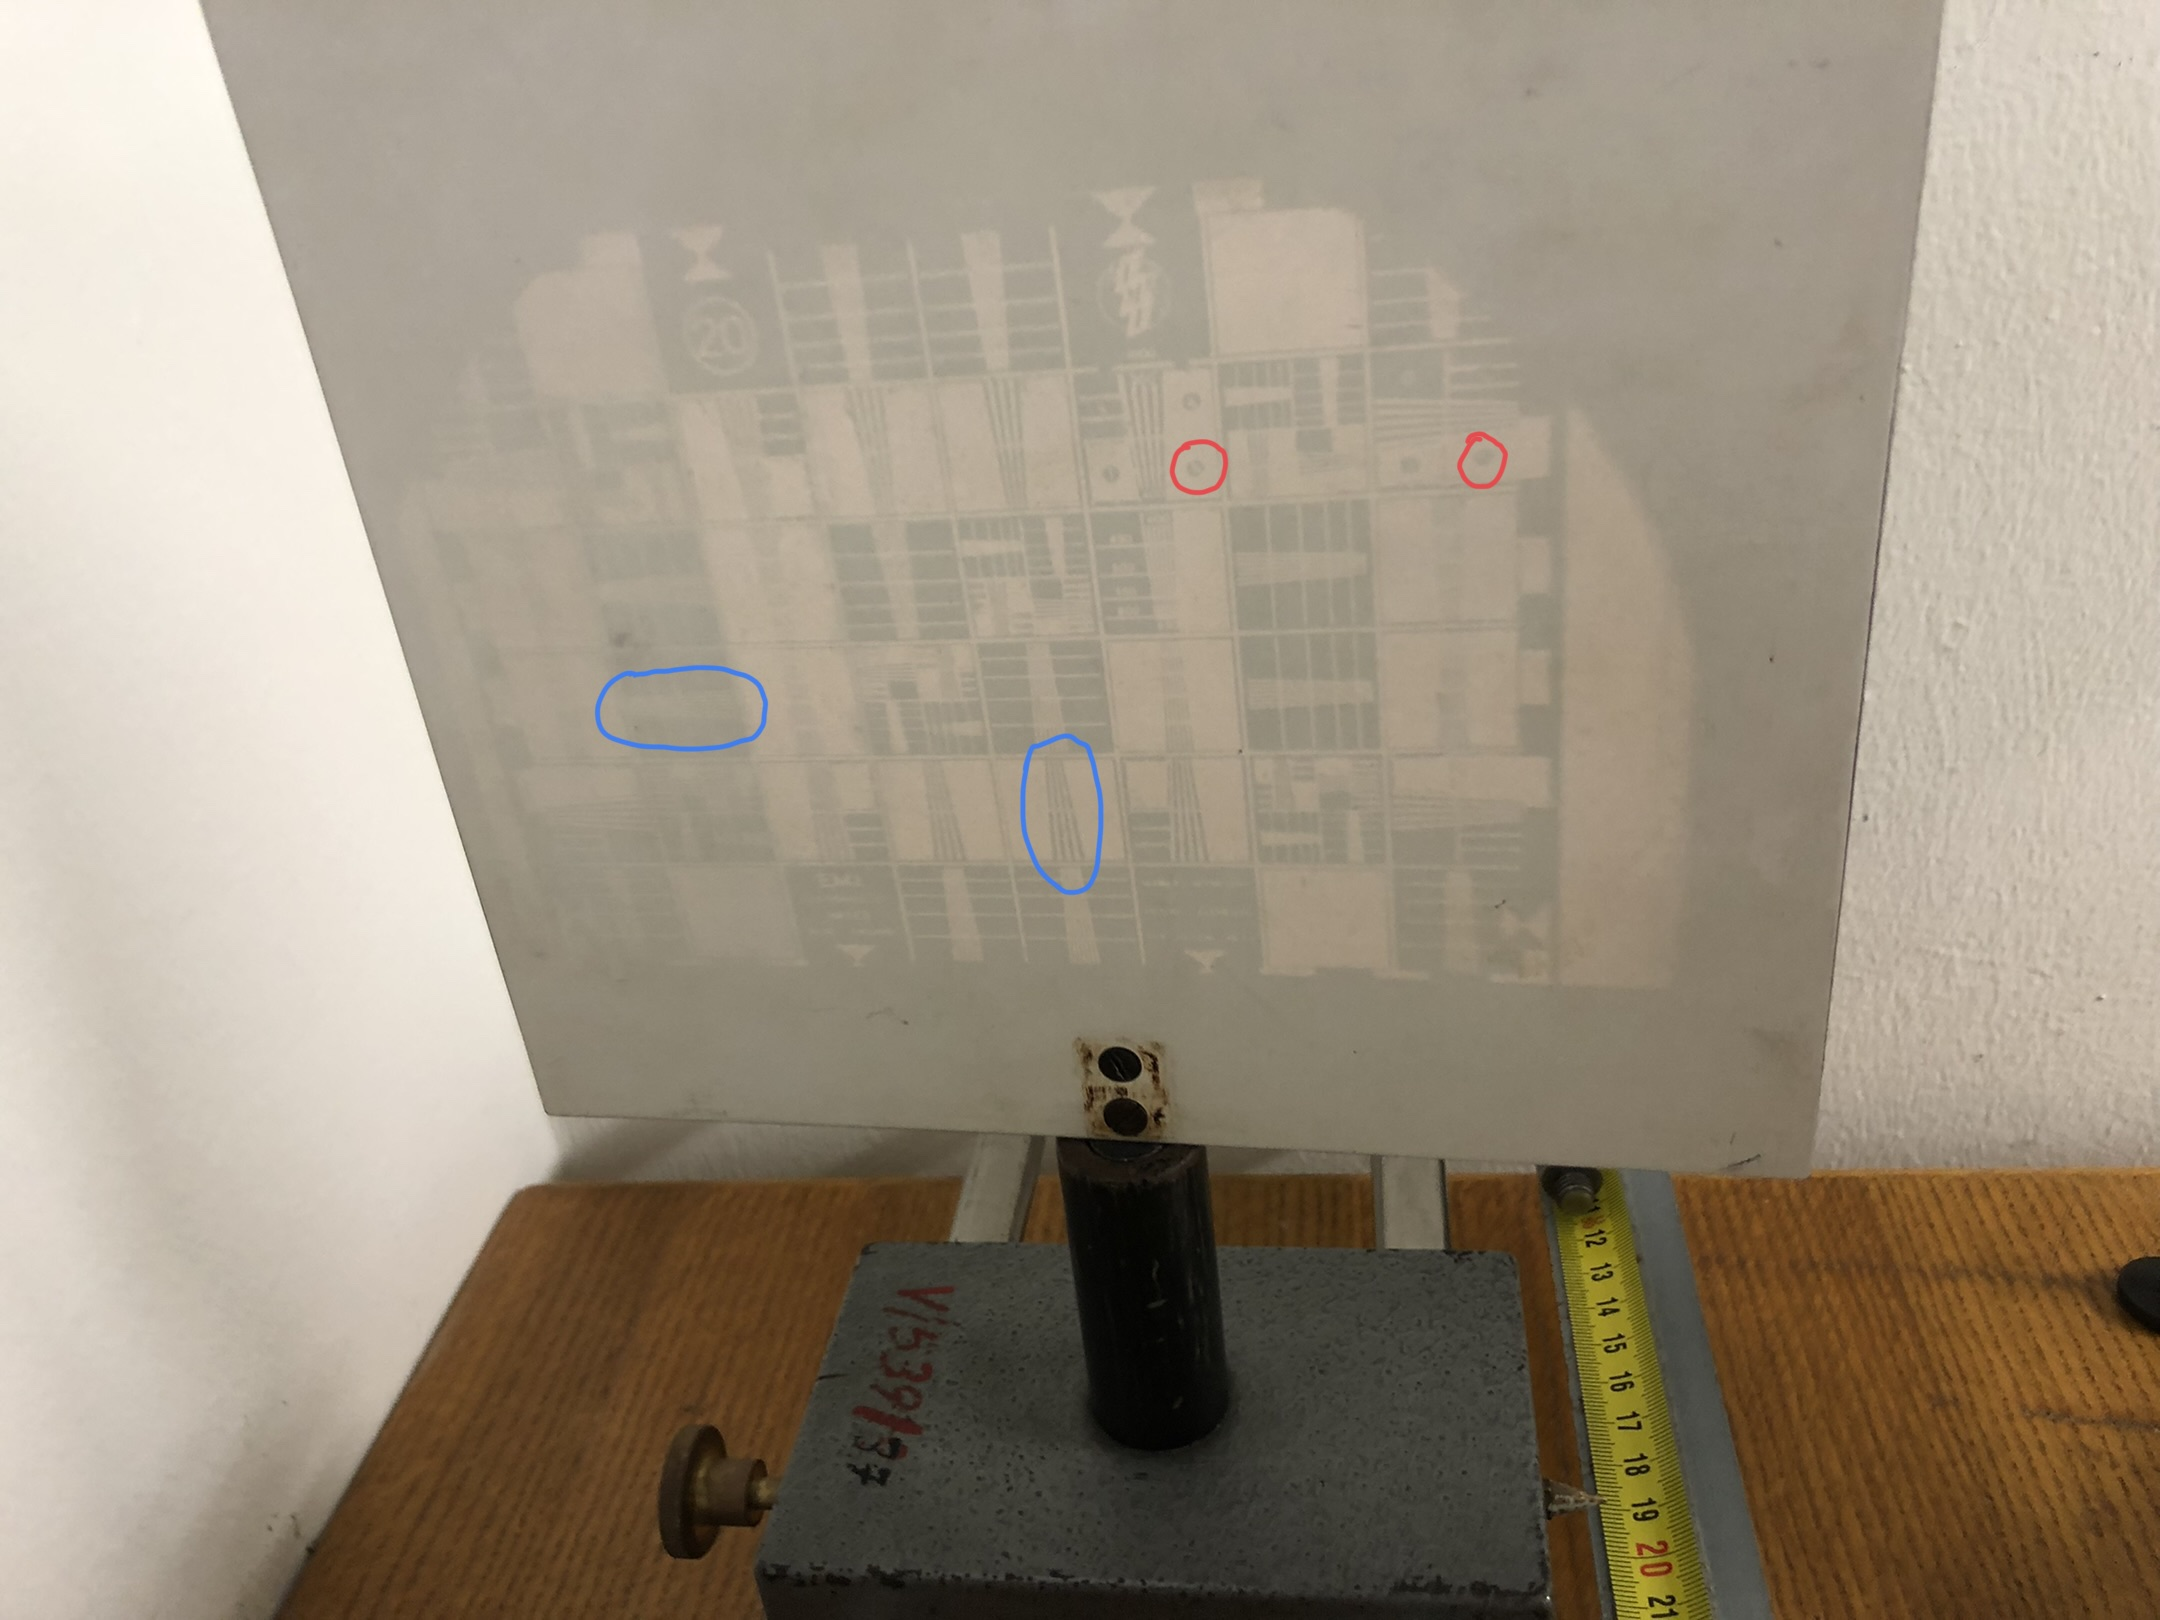
\includegraphics[width=\textwidth]{fehler}
		\captionbelowof{figure}{sichtbarer Fehler der spärischen Abberation und der Bildfeldwölbung}
		\label{fig:fehler}
	\end{minipage}
\end{center}
Vergleicht man hier beispielsweise außenliegendere Striche mit denen in der Mitte (in blau markiert), so stellt man fest, dass diese nicht so deutlich voneinander zu unterscheiden sind. Dies ist auch an den 0 zu erkennen (rot markiert).

\vspace{2mm}

Ein weiterer Abbildungsfehler ist das sogenannte Koma, welches beispielsweise
durch Neigen der Linse erreicht werden kann. \cite{demtroder2018ex2}

\newpage

\section{Zusammenfassung}

Im folgenden sind nochmals die wichtigsten Ergebnisse aufgelistet:

\vspace{2mm}

Für die Brennweite der Sammellinse nach der Laplace´schen Methode $f_{SL}$ ergibt sich folgender Wert:

\begin{align*}
	f_{SL} = \SI{24.2(8)}{\cm}
\end{align*}

\vspace{2mm}

Für die Brennweite der Sammellinse anhand des Plots $f_{SP}$ ergibt sich folgender Wert:

\begin{align*}
	f_{SP} = \SI{24.17(7)}{\cm}
\end{align*}

\vspace{2mm}

Für die Brennweite der Sammellinse nach der Bessel´schen Methode $f_{SB}$ ergibt sich folgender Wert:

\begin{align*}
	f_{SB} = \SI{25.0(13)}{\cm}
\end{align*}

\vspace{2mm}

Für die Brennweite der Zertreuungslinse $f_{Z}$ ergibt sich folgender Wert:

\begin{align*}
	f_{Z} = \SI{-14.2(13)}{\cm}
\end{align*}

\vspace{5mm}

\section{Anmerkungen}

Die ersten 3 Kapitel, sowie die dazugehörigen Abbildungen, wurden nicht von den
Autoren persönlich erstellt, sondern sind schon im Zuge der Aufgabenstellung,
in Form einer PDF, bereitgestellt und davon entnommen worden.
\cite{linsenvorlage}


\newpage

\printbibliography
\listoffigures
\listoftables
\end{document}



%Vorlagen
%

%Gleichungen werden so oder mit \begin{equation} formatiert

%Zitate
%\cite{erstes Wort}


%Unterdrücken von Einrücken
%\noindent 

%referenzen
% \aotoref{name}

%für Formeln $ f $
%\subsection{Idealisierungen}

%Gleichung

%\begin{equation}
%	k_{pos} = \frac{4}{300} \frac{V}{\mu\mathrm{s}} = 13333 \, \frac{V}{s}
%\end{equation}

%\begin{align}
%	 \ddot \phi -\frac{g}{l} \cdot \phi &=0 \label{eq:harm}\\
%     \frac{\text{d}^{2}}{\text{dt}^{2}} [\sin(\omega t)]  - \frac{g}{l} \cdot \sin(\omega t) &= 0 \\ 
%     \therefore \quad \omega^{2}&=\frac{g}{l} \label{eq:omega}
%\end{align}


%\begin{align}
%    T &= 2\pi \sqrt{\frac{l}{g}} \label{eq:reg_sqrt} \\
%    T^{2} &= \frac{4\pi^{2}}{g} l \label{eq:reg_lin} 
%\end{align}

%Kompliziertes Bild

%\begin{minipage}{\textwidth}
%\begin{minipage}[t]{0.43\textwidth}
%	\includegraphics[width=\textwidth]{pics/toplot.PNG}
%\end{minipage}
%\begin{minipage}[t]{0.45\textwidth}
%	\includegraphics[width=\textwidth]{pics/bottomlot.PNG}
%\end{minipage}
%	\captionof{figure}{Ansicht von Oben (Rechts) und von Unten (Links) des Senklots}
%	\label{fig:Senklot}
%    \vspace{1em}
%\end{minipage}



%\begin{minipage}{\textwidth}
%\begin{minipage}[t]{0.59\textwidth}
%    \centering
%    \includegraphics[width=\textwidth]{pics/Aufhangung.jpeg}
%    \captionbelowof{figure}{Aufhängung}
%    \label{fig:Aufhaengung}
%\end{minipage}
%\begin{minipage}[t]{0.40\textwidth}
%    \centering
%    \includegraphics[width=\textwidth]{pics/PendelAufbau.png}
%    \captionof{figure}{Versuchsaufbau}
%    \label{fig:Aufbau}
%\end{minipage}
%    \vspace{1em}
%\end{minipage}

%\begin{wrapfigure}[]{r}{0.4\textwidth}
%\begin{tabular}{@{}l@{}}
%\begin{minipage}{\textwidth}
%\includegraphics[width=0.38\textwidth]{pics/Aufhangung.jpeg}
%\noindent \captionbelowof{figure}{Aufhängung}
%\label{fig:Aufhaengung}
%\end{minipage}\\
%\begin{minipage}{\textwidth}
%\includegraphics[width=0.38\textwidth]{pics/PendelAufbau.png}
%\captionof{figure}{Versuchsaufbau}
%\label{fig:Aufbau}
%\end{minipage}
%\end{tabular}
%\end{wrapfigure}


%Tabelle

%\begin{align}
%	\Delta \bar T_{10} &= t \sigma_{\bar T_{10}} + \Delta T_{res} = \frac{t}{\sqrt{N}}\sigma_{T_{10}}+\Delta T_{res}\\
%	\Delta \bar T &= \frac{ \Delta \bar T_{10}}{10}
%\end{align}


%Tabelle
%
%\begin{table}[htbp]
%\centering
%\begin{tabular}{c|c|c|c|l}
%    [$\frac{\text{m}}{\text{s}^{2}}$] & Literaturwert & Wurzel Fit & Linearer Fit &\\ \hline
%    $g$ & \num{9.806191} & \num{9.79} & \num{9.80} &\\
%    $\Delta g$ & \num{1.2e-5} & \num{1e-2}& \num{1e-2} &\\
%\end{tabular}
%	\captionbelowof{table}{Vergleich mit Literaturwert}
%	\label{Tab:Vergleich}
%\end{table}


%\begin{align}
%	& \Delta T_{\phi} = 2\pi \sqrt{ \frac{l}{g} } \frac{\phi^{2}}{16} = 0.0052\,\text{s} 
%\end{align}
